\section{Ergebnisse und Diskussion}\label{chap:results}

In diesem Kapitel werden die Ergebnisse der einzelnen Zwischenschritte der Methodik nach \autoref{chap:Methodik} dargestellt und kritisch betrachtet.
Hierzu gehören die mit \gls{SIMBEV} simulierten Fahrtprofile und Standzeiten der \gls{EPKW}, sowie deren räumliche Verteilung und die Ergebnisse der Implementierung der verschiedenen Ladestrategien.
Abschließend erfolgt eine detaillierte Betrachtung der Ergebnisse der Netzuntersuchungen und der Ermittlung des Abregelungsbedarfs für die untersuchten Netze.


\subsection{Erzeugung und Charakteristik der Fahrtprofile}

Mit Hilfe des Software Tools \gls{SIMBEV} werden für die Referenznetzgebiete die Fahrtprofile der im \gls{MS}-Netzgebiet befindlichen \gls{EPKW} erstellt.
Die Charakteristik der Fahrtprofile spielt eine entscheidende Rolle für die Wirksamkeit der Ladestrategien und die Auswirkungen auf die \gls{MS}-Netzgebiete.
Hierbei steht vor allem die Jahresfahrleistung der \glspl{EPKW}, der Anteil flexibilisierbarer und nicht-flexibilisierbare Ladevorgänge, die Gleichzeitigkeit und zeitliche Verteilung der Ladevorgänge im Vordergrund.
Innerhalb dieses Kapitels werden die Ergebnisse der Regionalisierung dargestellt, sowie die Charakteristik der erzeugten Fahrtprofile kritisch betrachtet.
Dabei liegt der Fokus auf der Überprüfung der Plausibilität der Fahrtprofile und dem herausstellen des Flexibilisierungspotentials von Ladevorgängen von \gls{EPKW}.\medskip

Die Ermittlung der Anzahl der Fahrzeuge erfolgt nach \autoref{chap:simbev_theo} auf Gemeindeebene.
In der Regel liegen innerhalb eines \gls{MS}-Netzgebietes mehrere Gemeinden und insgesamt liegen \num{34} Gemeinden innerhalb der fünf Referenznetzgebiete.
Die Auswertung ergibt die Anzahl der simulierten Fahrzeuge nach \autoref{tab:car_count} je Fahrzeugtyp und Szenario.
Zusätzlich findet sich im Anhang in \autoref{tab:car_count_long} eine detailliertere Darstellung je Fahrzeugtyp, -klasse und Szenario.

{
\renewcommand{\arraystretch}{1.2}% grßerer Zeilenabstand
\sisetup{range-phrase=~{--}~}% Gedankenstrich statt "bis" bei SIrange
\begin{table}[H]
	\begin{center}
		\caption{Anzahl der Fahrzeuge in den Gemeinden der Referenznetzgebiete je Typ und Szenario}
		\begin{tabu} to 0.6\textwidth {X[1.2] X[1, r] X[1, r] X[1, r]}
			\toprule
			Szenario         & BEV         & PHEV        & Summe       \\ \midrule
			NEP C~\num{2035} & \num{14270} & \num{8841}  & \num{23111} \\
			Referenz         & \num{25545} & \num{15826} & \num{41371} \\
			Antriebswende    & \num{48617} & \num{30117} & \num{78734} \\ \bottomrule
		\end{tabu}
		\label{tab:car_count}
	\end{center}
	\vspace{-3mm}%Put here to reduce too much white space after your table
\end{table}
}

Die \num{34} Gemeinden weisen drei der sieben \gls{REGIOSTAR} (vgl. \autoref{tab:RegioStaR}) auf.
Hierzu zählen der kleinstädtische, dörfliche Raum einer ländlichen Region (\gls{ID} \num{77}), Mittelstädte im städtischen Raum (\gls{ID} \num{76}) und Mittelstädte im städtischen Raum einer Stadtregion (\gls{ID} \num{73}).
Die Jahresfahrleistung der simulierten \glspl{BEV} je \gls{REGIOSTAR} wurde zusammenfassend über alle Szenarien hinweg berechnet und findet sich in \autoref{tab:bev_distance}.
Dabei zeigt sich, dass in \gls{ID} \num{77} im Schnitt die weitesten Strecken zurückgelegt werden, welches den Erwartungen nach \gls{MID} \cite{Nobis2019} entspricht.
Jedoch liegen die Jahresfahrleistungen insgesamt unter den Angaben des \gls{MID} von durchschnittlich \SI{14700}{\km}, aber auf einem ähnlichen Niveau zu einer Auswertung von Kfz-Versicherungen des Vergleichsportals \textit{Check24} \cite{CHECK24GmbH2018}, wonach die durchschnittliche Jahresfahrleistung in Deutschland im Jahr \num{2017} bei \SI{11888}{\km} lag.
Insgesamt spiegeln die Jahresfahrleistungen \glspl{SIMBEV} somit ein progressives Szenario mit einer sinkenden Jahresfahrleistung wider.


{
\renewcommand{\arraystretch}{1.2}% grßerer Zeilenabstand
\sisetup{range-phrase=~{--}~}% Gedankenstrich statt "bis" bei SIrange
\begin{table}[H]
	\begin{center}
		\caption{Durchschnittliche Jahresfahrleistung mit Standardabweichung und maximale Jahresfahrleistung von BEVs je untersuchter RegioStaR 7 Raumtypologie}
		\begin{tabu} to 0.8\textwidth {X[0.2] X[1.6, r] X[1.5, r]}
			\toprule
			ID 	   				   & Durchschnittle Jahresfahrleistung                  & Maximale Jahresfahrleistung \\ \midrule
			\num{73}               & \SI[separate-uncertainty = true]{11660(6408)}{\km} & \SI{58575}{\km}             \\
			\num{76}               & \SI[separate-uncertainty = true]{11500(6243)}{\km} & \SI{54204}{\km}             \\
			\num{77}               & \SI[separate-uncertainty = true]{12353(6395)}{\km} & \SI{55426}{\km}             \\ \bottomrule
		\end{tabu}
		\label{tab:bev_distance}
	\end{center}
	\vspace{-3mm}%Put here to reduce too much white space after your table
\end{table}
}

Eine Betrachtung der durchschnittlichen Stand- und Ladezeiten von Ladevorgängen bei maximal möglicher Ladeleistung des Ladevorgangs je Wegezweck in \autoref{tab:StandingTime} zeigt, dass die \gls{EPKW} im privaten Bereich einen Großteil der Standzeit nicht geladen werden.
So macht die durchschnittliche Ladezeit der Wegezwecke \nH und \Arbeit nur etwa \SI{8}{\percent} der Standzeit aus, welches das erhebliche Flexibilisierungspotential der Ladevorgänge deutlich macht.

{
\renewcommand{\arraystretch}{1.2}% grßerer Zeilenabstand
\sisetup{range-phrase=~{--}~}% Gedankenstrich statt "bis" bei SIrange
\begin{table}[H]
	\begin{center}
		\caption{Durchschnittliche Stand- und Ladezeiten von Ladevorgängen je Wegezweck mit Standardabweichung}
		\begin{tabu} to 0.8\textwidth {X[0.5] X[1, r] X[1, r]}
			\toprule
			Wegezweck  & Durchschnittliche Standzeit                      & Durchschnittliche Ladezeit	                     \\ \midrule
			Arbeit     & \SI[separate-uncertainty = true]{7.3(37)}{\hour} & \SI[separate-uncertainty = true]{0.6(5)}{\hour}  \\
%			dienstlich & \SI[separate-uncertainty = true]{4.4(58)}{\hour} & \SI[separate-uncertainty = true]{1.1(7)}{\hour}  \\
%			Ausbildung & \SI[separate-uncertainty = true]{6.2(39)}{\hour} & \SI[separate-uncertainty = true]{1.4(11)}{\hour} \\
%			Einkauf    & \SI[separate-uncertainty = true]{2.1(38)}{\hour} & \SI[separate-uncertainty = true]{0.8(5)}{\hour}  \\
%			Erledigung & \SI[separate-uncertainty = true]{4.2(56)}{\hour} & \SI[separate-uncertainty = true]{0.9(6)}{\hour}  \\
%			Freizeit   & \SI[separate-uncertainty = true]{6.0(62)}{\hour} & \SI[separate-uncertainty = true]{1.1(7)}{\hour}  \\
			nach Hause & \SI[separate-uncertainty = true]{8.9(57)}{\hour} & \SI[separate-uncertainty = true]{0.7(6)}{\hour}  \\ \bottomrule
		\end{tabu}
		\label{tab:StandingTime}
	\end{center}
	\vspace{-3mm}%Put here to reduce too much white space after your table
\end{table}
}

Der Anteil flexibilisierbarer Ladevorgänge entspricht dem Anteil am Gesamtenergiebedarf der \glspl{EPKW}, der an privaten Ladepunkten der \UCs \zH oder \Firmeparkplatz nachgeladen wird.
Zusätzlich sind nur Ladevorgänge flexibilisierbar, deren Standzeit größer ist als die Mindestladedauer.
Demgegenüber stehen nicht-flexibilisierbare Ladevorgänge im öffentlichen Raum und an Schnellladestationen bzw. Ladevorgänge deren Standzeit der Mindestladedauer entspricht.
Im Mittel liegt der Anteil flexibilisierbarer Ladevorgänge über alle Szenarien je Gemeinde bei \SI{71.1}{\percent}.
Hiervon ausgenommen ist die \SzeFirmenparkplatzdot, bei der es aufgrund des geringeren Bestands an Ladeinfrastruktur des \UC \Firmeparkplatz zu mehr Ladevorgängen im öffentlichen Raum kommt.
Der Anteil flexibilisierbarer Ladevorgänge liegt bei der Szenarette bei \SI{66.1}{\percent}.
In \autoref{tab:ChargingShare} sind die Anteile flexibilisierbarer und nicht-flexibilisierbarer Ladevorgänge zusammengefasst.

{
\renewcommand{\arraystretch}{1.2}% grßerer Zeilenabstand
\sisetup{range-phrase=~{--}~}% Gedankenstrich statt "bis" bei SIrange
\begin{table}[H]
	\begin{center}
		\caption{Aufteilung in flexibiliserbare und nicht-flexibiliserbare Ladevorgänge nach dem Anteil vom Gesamtenergiebedarf der E-Pkw je Gemeinde mit Standardabweichung}
		\begin{tabu} to 0.9\textwidth {X[1] X[1.3, r] X[1, r]}
			\toprule
								  					& \SzeFirmenparkplatzdot                               & Sonstige Szenarien                                   \\ \midrule
			Flexibilisierbar       	& \SI[separate-uncertainty = true]{66.1(23)}{\percent} & \SI[separate-uncertainty = true]{71.1(23)}{\percent} \\
			Nicht-flexibilisierbar 	& \SI[separate-uncertainty = true]{33.9(23)}{\percent} & \SI[separate-uncertainty = true]{28.9(23)}{\percent} \\ \bottomrule
		\end{tabu}
		\label{tab:ChargingShare}
	\end{center}
	\vspace{-3mm}%Put here to reduce too much white space after your table
\end{table}
}

In \autoref{fig:example_load_profile} findet sich beispielhaft das \gls{EPKW}-Lastprofil für das Referenz-Laden im Netz \(176_{\text{PV}}\) über eine Woche im Antriebswende-Szenario (links).
Zusätzlich ist das \gls{EPKW}-Lastprofil der gleichen Gemeinde in der \SzeFirmenparkplatz (rechts) dargestellt.

\begin{figure}[H]
    \centering
    \includegraphics[width=\textwidth]{Bilder/example_load_profile}
    \caption[E-Pkw-Lastprofil für Referenz-Laden im Netz \num{176} der simulierten Woche im Antriebswende-Szenario und der Sensitivität Firmenparkplatz]{E-Pkw-Lastprofil (netzseitige Last; inkl. Umwandlungsverluste) für Referenz-Laden im Netz \(176_{\text{PV}}\) der simulierten Woche im Antriebswende-Szenario (links) und der \SzeFirmenparkplatz (rechts)}\label{fig:example_load_profile}
\end{figure}

Die Lastgänge der \UCs \zH und \Firmeparkplatz entsprechen den Ladevorgängen im privaten Bereich.
Die verbleibenden \UCsdot, mit Ausnahme der Schnellladevorgänge (\gls{HPC}), werden unter dem \UC \oeffen zusammengefasst.
Deutlich zu erkennen ist die hohe Gleichzeitigkeit am Vormittag aufgrund des Wegezwecks \Arbeitdot.
Auch die Rückkehr zum Wohnort ist ab dem frühen Nachmittag in den Lastgängen der \UCs \zH und \oeffen klar zu erkennen.
Weiterhin kommt es ab mittags zu mehr Fahrten der Wegezwecke \Einkaufdot, \Erledigung und \Freizeitdot, welche sich ebenfalls in dem Lastgang des \UC \oeffen niederschlagen.
Schnellladevorgänge treten unregelmäßig im Verlauf der Woche auf.
Vor allem am Sonntag kommt es zu geringeren Anteilen von Ladevorgängen der \UCs \zH und \Firmeparkplatzdot, wodurch das Flexibilisierungspotential am Wochenende geringer ausfällt.
Gegenüber dem Antriebswende-Szenario sinkt die Höchstlast in der \SzeFirmenparkplatzdot.
Jedoch sinkt auch das Flexibilisierungspotential bei einem annähernd gleichbleibendem Energiebedarf durch die Verschiebung der Ladevorgänge in den öffentlichen Raum.\medskip

Die entsprechenden Dauerlastkurven für die Gemeinde über eine Woche nach \autoref{fig:example_load_curve} zeigen deutlich die dominante Rolle der Hochlastphase, die aufgrund der hohen Gleichzeitigkeit des Wegezwecks \Arbeit in den \UCs \Firmeparkplatz und \Straszenrand auftritt.
So wird im Antriebswende-Szenario eine Spitzenlast von \SI{14.8}{\mw} erreicht und in der \SzeFirmenparkplatz von nur \SI{11.3}{\mw}.
Dem Netz \(176_{\text{PV}}\) werden im Antriebswende-Szenario \SI{26359}{\FZ} zugeordnet, welches einem Verhältnis von Spitzenlast zu Fahrzeugen von \SIrange[range-phrase=~bzw.~]{0.56}{0.43}{\kWperFZ} entspricht.
Zum Vergleich wurde in der \textit{Kurzstudie Elektromobilität} für den \gls{NEP} \cite{Ebner2019} für \SI{12}{\MioStk} innerhalb eines Jahres eine Spitzenlast von \SI{12}{\gw} ermittelt, welches einem Verhältnis von \SI{1.00}{\kWperFZ} entspricht.
Für eine mittlere Woche liegt die Spitzenlast in der \textit{Kurzstudie Elektromobilität} bei \SI{9}{\gw} und somit bei \SI{0.75}{\kWperFZ}.
Die Spitzenlast wird nach der \textit{Kurzstudie Elektromobilität} in der Regel am Nachmittag erreicht, da im Vergleich zu dieser Arbeit mehr Ladevorgänge des \UC \zH und weniger Ladevorgänge des \UC \Firmeparkplatz stattfinden.
Hierdurch ergibt sich innerhalb der Woche am Abend eine hohe Gleichzeitigkeit des \UC \zHdot, während in der durchgeführten Simulation dieser Arbeit täglich zwei Leistungsspitzen mit einer insgesamt geringeren Gleichzeitigkeit am Morgen und am Nachmittag auftreten.
Die Ergebnisse der Simulation liegen somit in einer ähnlichen Dimension.

\begin{figure}[H]
    \centering
    \includegraphics[width=\textwidth]{Bilder/example_load_duration_curve}
    \caption[E-Pkw-Dauerlastkurve für Referenz-Laden im Netz \num{176} über eine Woche im Antriebswende-Szenario und der Sensitivität Firmenparkplatz]{E-Pkw-Dauerlastkurve (netzseitige Last; inkl. Umwandlungsverluste) für Referenz-Laden im Netz \(176_{\text{PV}}\) über eine Woche im Antriebswende-Szenario (oben) und der \SzeFirmenparkplatz (unten)}\label{fig:example_load_curve}
\end{figure}

Zum Zeitpunkt der Erstellung der Fahrtprofile ist es noch nicht möglich, einen längeren Zeitraum als eine Woche am Stück zu simulieren.
Durch die Zuordnung eines zufälligen Eingangs-\gls{SOC} für einige Fahrzeuge (s. \autoref{chap:simbev_theo}) kann das Initialproblem eines geringen Ladebedarfs des \UC \Firmeparkplatz am Montag behoben werden.
Jedoch kann hierdurch ein weiterer Effekt nicht verhindert werden.
Bei Fahrzeugen, welche weder einen festen Ladepunkt für den \UC \zH oder \Firmeparkplatz zugewiesen bekommen, fällt der \gls{SOC} im Laufe der Woche im Mittel langsam ab.
Hierdurch kommt es durch die Abhängigkeit der Ladewahrscheinlichkeit vom \gls{SOC} zu einer Zunahme des Ladebedarfs im öffentlichen Raum im Verlaufe der Woche.
Es ist zu vermuten, dass dies weiterhin dazu führt, dass Ladevorgänge an Schnellladeinfrastruktur un­ter­re­prä­sen­tiert dargestellt werden.


\subsection{Verteilung der Ladevorgänge auf die Ladeinfrastruktur}\label{chap:distribute_demand_ev}

Innerhalb dieses Kapitels werden die Ergebnisse der Verteilung der Ladevorgänge auf konkrete Ladestationen beschrieben.
Hierbei soll vor allem herausgestellt werden, wie sich der Ladebedarf auf die Spannungsebenen verteilt und ob es zu starken lokalen Konzentrationen des Ladebedarfs kommt.\medskip

Die Ermittlung der möglichen Anschlusspunkte nach \autoref{chap:theo_distribution} liefert je \gls{MS}-Netzgebiet eine große Anzahl an möglichen Netzanschlusspunkten.
Den ermittelten Anschlusspunkten werden zufällig und gewichtet Ladepunkte und -vorgänge zugeordnet, um die Anschlussleistung des Anschlusspunktes zu bestimmen und den Ladebedarf zu regionalisiern.
In \autoref{fig:cps_in_grid} finden sich beispielhaft die ermittelten und zugewiesenen Netzanschlusspunkte für Ladeinfrastruktur innerhalb des Netzes \(176_{\text{PV}}\) für das Antriebswende-Szenario.
Hierbei erfolgt eine Einteilung in die \UCs \zHdot, \Firmeparkplatzdot, \oeffen und \gls{HPC}.
Es wird deutlich, dass die Ladeinfrastruktur des \UC \zH die meisten Netzanschlusspunkte aufweist, während für die Schnellladeinfrastruktur nur wenige Netzanschlusspunkte benötigt werden.

\begin{figure}[H]
    \centering
    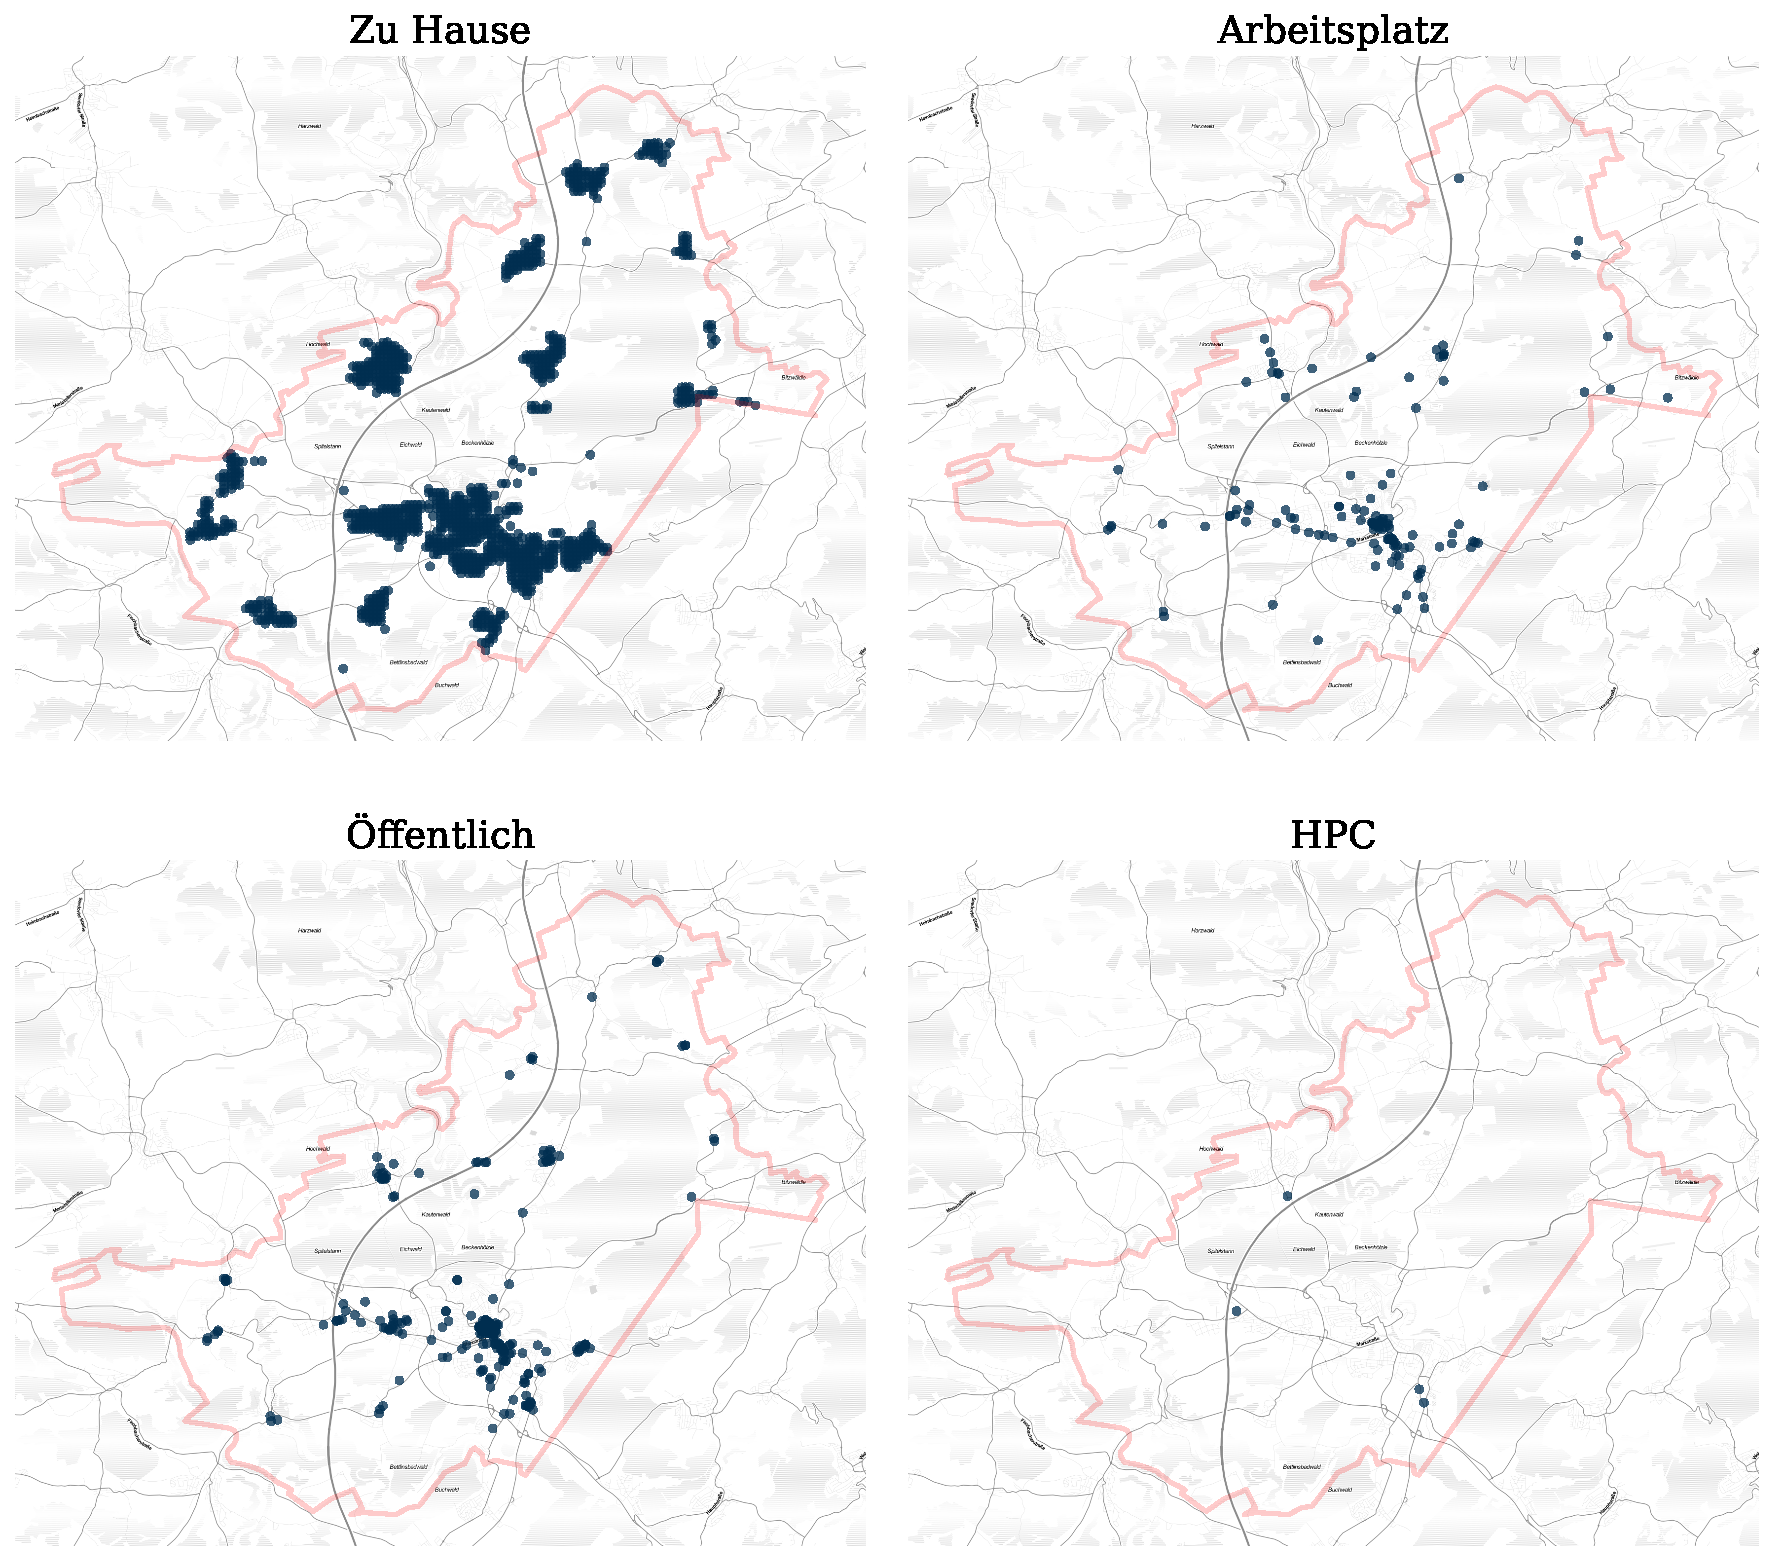
\includegraphics[width=\textwidth]{Bilder/cps_in_grid_176}
    \caption[Geographische Verteilung der ermittelten Netzanschlusspunkte für Ladeinfrastruktur im Netz \num{176} für das Antriebswende-Szenario je Lade Use Case]{Geographische Verteilung der ermittelten Netzanschlusspunkte für Ladeinfrastruktur im Netz \(176_{\text{PV}}\) für das Antriebswende-Szenario je Lade Use Case}\label{fig:cps_in_grid}
\end{figure}

Neben der geographischen Lokalisation der Ladeinfrastruktur ist es für die Netzuntersuchungen entscheidend, ob die Ladeinfrastruktur in der \gls{NS}- oder \gls{MS}-Ebene angeschlossen wird.
Erfolgt der Anschluss in der \gls{NS}-Ebene, dann werden sowohl die Betriebsmittel der \gls{NS}- und \gls{MS}-Ebene belastet, während bei einem Anschluss in der \gls{MS}-Ebene auch nur diese betroffen ist.
Außerdem findet bei einem Anschluss von privater Ladeinfrastruktur in der \gls{MS}-Ebene auch bei der Referenz-Ladestrategie reduziertes Laden statt (s. \autoref{chap:theo_strategies}).
In \autoref{tab:lvConnectionShare} findet sich der Anteil des in der \gls{NS}-Ebene anfallenden Energiebedarfs vom Gesamtenergiebedarf der Ladeinfrastruktur im \gls{MS}-Netzgebiet.
Mit einer steigenden Zahl von Fahrzeugen steigt auch der Anteil von Ladeinfrastruktur in der \gls{MS}-Ebene, da eine steigende Anzahl von Ladepunkten auf eine gleichbleibende Anzahl von möglichen Anschlusspunkten verteilt werden muss und somit die kumulierte Leistung der Ladestationen zunimmt.
Gleichzeitig zeigt sich, dass in der \SzeFirmenparkplatz der Anteil von Ladeinfrastruktur in der \gls{MS}-Ebene deutlich geringer ausfällt als im Antriebswende-Szenario, trotz der gleichen Anzahl an \gls{EPKW}.
Dies lässt sich damit erklären, dass neben der öffentlichen Ladeinfrastruktur vor allem Ladeinfrastruktur des \UC \Firmeparkplatz einen Anschluss in der \gls{MS}-Ebene benötigt.
Da im Antriebswende-Szenario mehr Ladevorgänge des Wegezwecks \Arbeit auf eine gleichbleibende Anzahl von möglichen Anschlusspunkten für Ladeinfrastruktur des \UC \Firmeparkplatz verteilt werden müssen, fällt die Anschlussleistung dieser Ladeinfrastruktur im Schnitt höher aus und macht somit einen Anschluss in der \gls{MS}-Ebene nötig.

{
\renewcommand{\arraystretch}{1.2}% grßerer Zeilenabstand
\sisetup{range-phrase=~{--}~}% Gedankenstrich statt "bis" bei SIrange
\begin{table}[H]
	\begin{center}
		\caption{Anteil des in der NS-Ebene anfallenden Energiebedarfs vom Gesamtenergiebedarf der Ladeinfrastruktur je Szenario}
		\begin{tabu} to \textwidth {X[0.5] X[1, r] X[1, r] X[1.2, r] X[1.2, r]}
			\hline
			Netz ID    & NEP C \num{2035}    & Referenz            & Antriebswende       & \glqq Firmenparkplatz\grqq \\ \hline
			\num{176}  & \SI{98.0}{\percent} & \SI{92.9}{\percent} & \SI{82.0}{\percent} & \SI{91.3}{\percent}        \\
			\num{177}  & \SI{96.6}{\percent} & \SI{86.8}{\percent} & \SI{77.8}{\percent} & \SI{86.7}{\percent}        \\
			\num{1056} & \SI{99.8}{\percent} & \SI{99.5}{\percent} & \SI{94.0}{\percent} & \SI{97.9}{\percent}        \\
			\num{1690} & \SI{99.8}{\percent} & \SI{97.0}{\percent} & \SI{86.5}{\percent} & \SI{92.9}{\percent}        \\
			\num{1811} & \SI{99.9}{\percent} & \SI{98.7}{\percent} & \SI{90.0}{\percent} & \SI{95.2}{\percent}        \\
			\num{2534} & \SI{99.7}{\percent} & \SI{97.4}{\percent} & \SI{80.8}{\percent} & \SI{91.4}{\percent}        \\ \hline
		\end{tabu}
		\label{tab:lvConnectionShare}
	\end{center}
	\vspace{-3mm}%Put here to reduce too much white space after your table
\end{table}
}

In \autoref{tab:largestLVGridShare} ist die Anzahl an \gls{NS}-Netzen je \gls{MS}-Netzgebiet und der maximale Anteil eines \gls{NS}-Netzes am Gesamtenergiebedarf der Ladeinfrastruktur in der \gls{NS}-Ebene in allen betrachteten Szenarien dargestellt.
Hierbei wird deutlich, dass es in einigen \gls{MS}-Netzgebieten zu einer starken lokalen Konzentration an Ladeinfrastruktur kommt.
So fallen beispielsweise im Netz \(176_{\text{PV}}\) im \gls{NEP} C~\num{2035} Szenario \SI{36.3}{\percent} des Energiebedarfs der Ladeinfrastruktur in der \gls{NS}-Ebene innerhalb eines einzigen \gls{NS}-Netzes an.
Diese starke Konzentration spiegelt sich in \autoref{fig:cps_in_grid} durch eine starke Konzentration der Ladeinfrastruktur in den bewohnten Regionen wider.
In der Realität würde es bei solch starken lokalen Konzentrationen vermutlich zu einem Netzneubau kommen, welcher innerhalb dieser Arbeit nicht abgebildet werden kann.

{
\renewcommand{\arraystretch}{1.2}% grßerer Zeilenabstand
\sisetup{range-phrase=~{--}~}% Gedankenstrich statt "bis" bei SIrange
\begin{table}[H]
	\begin{center}
		\caption{Anzahl der NS-Netze je MS-Netzgebiet und maximal anfallender Energieanteil eines NS-Netzes am Gesamtenergiebedarf der Ladeinfrastruktur in den NS-Netzen mit Standardabweichung je MS-Netzgebiet und Szenario}
		\begin{tabu} to 0.8\textwidth {X[0.5] X[1, r] X[2, r]}
			\hline
			Netz ID    & Anzahl NS-Netze & Maximaler Ladeanteil eines NS-Netzes                 \\ \hline
			\num{176}  & \num{105}       & \SI[separate-uncertainty = true]{34.7(12)}{\percent} \\
			\num{177}  & \num{56}        & \SI[separate-uncertainty = true]{25.5(8)}{\percent}  \\
			\num{1056} & \num{130}       & \SI[separate-uncertainty = true]{12.3(7)}{\percent}  \\
			\num{1690} & \num{179}       & \SI[separate-uncertainty = true]{11.2(1)}{\percent}  \\
			\num{1811} & \num{381}       & \SI[separate-uncertainty = true]{7.4(3)}{\percent}   \\
			\num{2534} & \num{9}         & \SI[separate-uncertainty = true]{61.1(7)}{\percent}  \\ \hline
		\end{tabu}
		\label{tab:largestLVGridShare}
	\end{center}
	\vspace{-3mm}%Put here to reduce too much white space after your table
\end{table}
}


\subsection{Auswirkungen der Ladestrategien}\label{chap:results_charging_strategies}

Innerhalb dieses Kapitels soll der Einfluss der Ladestrategien auf die Spitzenlast im Last- und Rückspeisefall aufgezeigt werden.
Zusätzlich wird die Veränderung der Lastprofile des Ladebedarfs der \gls{EPKW} aufgrund der Ladestrategien dargestellt.
Im Rahmen der Netzuntersuchungen kommt den Zeitreihen der Last der \glspl{EPKW} die größte Bedeutung zu, da die Last und Erzeugung aller anderen Verbraucher und Erzeuger nicht variiert wird.
Das Ziel der Ladestrategien (s. \autoref{chap:theo_strategies}) ist es, die Netzbelastung möglichst gering zu halten.
Bei den Ladegruppen und dem reduzierten Laden soll dies durch ein präventives Lademanagement und bei dem Residuallast-Laden durch ein aktives Lademanagement erreicht werden.

\begin{figure}[H]
    \centering
    \includegraphics[width=1\textwidth]{Bilder/example_resiual_load}
    \caption[Residuallast über ein Jahr im Netz \num{176} für das Antriebswende-Szenario]{Residuallast über ein Jahr im Netz \(176_{\text{PV}}\) für das Antriebswende-Szenario}\label{fig:residual_load}
\end{figure}

\autoref{fig:residual_load} stellt beispielhaft die Residuallast im Netz \(176_{\text{PV}}\) in Abhängigkeit von der Ladestrategie im Antriebswende-Szenario dar.
Es zeigt sich deutlich, dass nur die Residuallast-Ladestrategie zu einer Glättung der Residuallastkurve führt.
Dies bestätigt sich in einer Betrachtung der Veränderung der Spreizung zwischen dem maximalen Last- und Rückspeisefall in den Referenznetzgebieten aufgrund der Ladestrategien in \autoref{tab:ResidualLoadSpread}.
Demnach kann durch die Residuallast-Ladestrategie die Spreizung vor allem in den \gls{PV}- und Last-domninierten Netzen stark reduziert werden.
In den Wind-dominierten Netzen fällt die Reduktion geringer aus, da das Verhältnis zwischen Einspeisung und Ladebedarf größer ausfällt und damit der Einfluss des Ladebedarfs auf die Residuallast abnimmt.
Die präventiven Ladestrategien zeigen hingegen keinen deutlichen Einfluss auf die Residuallast in den Referenznetzgebieten.
In der Regel führen die präventiven Ladestrategien gegenüber dem Referenz-Laden sogar zu einer leichten Erhöhung der Spreizung.
Hierbei kommt es bei den Ladegruppen eher zu einer Erhöhung der Last im Lastfall, während es durch das reduzierte Laden zu einer Erhöhung im Rückspeisefall kommt, wobei auf diesen Effekt detailliert in \autoref{chap:cur_results} eingegangen wird .

{
\renewcommand{\arraystretch}{1.2}% grßerer Zeilenabstand
\sisetup{range-phrase=~{--}~}% Gedankenstrich statt "bis" bei SIrange
\begin{table}[H]
	\begin{center}
		\caption{Spreizung der Residuallast zwischen dem maximalen Last- und Rückspeisefall in den Referenznetzgebieten und die prozentuale Veränderung der Spreizung aufgrund der Ladestrategien im Antriebswende-Szenario}
		\begin{tabu} to \textwidth {X[0.5] X[1, r] X[1, r] X[1.2, r] X[1.2, r]}
			\toprule
			Netz ID    & Referenz-Laden  & Ladegruppen                               & Reduziertes Laden                          & Residuallast-Laden                         \\ \midrule
			\(176_{\text{PV}}\)  & \SI{58.4}{\mw}  & \SI[retain-explicit-plus]{+5.3}{\percent} & \SI[retain-explicit-plus]{+3.6}{\percent}  & \SI[retain-explicit-plus]{-24.0}{\percent} \\
			\(1056_{\text{PV}}\) & \SI{84.5}{\mw}  & \SI[retain-explicit-plus]{+0.0}{\percent} & \SI[retain-explicit-plus]{+0.6}{\percent}  & \SI[retain-explicit-plus]{-10.2}{\percent} \\
			\(1690_{\text{W}}\) & \SI{113.5}{\mw} & \SI[retain-explicit-plus]{+0.1}{\percent} & \SI[retain-explicit-plus]{+0.8}{\percent}  & \SI[retain-explicit-plus]{-5.7}{\percent}  \\
			\(1811_{\text{W}}\) & \SI{98.4}{\mw}  & \SI[retain-explicit-plus]{+0.3}{\percent} & \SI[retain-explicit-plus]{+0.4}{\percent}  & \SI[retain-explicit-plus]{-7.0}{\percent}  \\
			\(177_{\text{L}}\)  & \SI{36.6}{\mw}  & \SI[retain-explicit-plus]{+4.5}{\percent} & \SI[retain-explicit-plus]{-0.2}{\percent}  & \SI[retain-explicit-plus]{-25.5}{\percent} \\ \bottomrule
		\end{tabu}
		\label{tab:ResidualLoadSpread}
	\end{center}
	\vspace{-3mm}%Put here to reduce too much white space after your table
\end{table}
}

In \autoref{fig:residual_load_diff} ist die Veränderung der Last der \glspl{EPKW} im Netz \(176_{\text{PV}}\) über ein Jahr in Abhängigkeit von den verschiedenen Ladestrategien dargestellt.
Dabei zeigt die Darstellung der Referenz-Ladestrategie (oben links) die Last der \glspl{EPKW} über ein Jahr, während in den anderen drei Darstellungen die Differenz der jeweiligen Ladestrategie zum Referenz-Laden abgebildet wird.
Da im Antriebswende-Szenario im Netz \(176_{\text{PV}}\) \SI{18}{\percent} des Ladebedarfs in der \gls{MS}-Ebene anfallen (vgl. \autoref{tab:lvConnectionShare}), kommt es beim Referenz-Laden bereits zu einem erhöhten Anteil an reduzierten Ladevorgängen.
Hiervon ist vor allem der \UC \Firmeparkplatz und nur selten der \UC \zH betroffen.
Bei den Ladegruppen werden die Ladevorgänge zeitlich weniger gestreckt als bei reduzierten Ladevorgängen, weshalb gegenüber dem Referenz-Laden eine Zunahme der Last am Morgen festzustellen ist.
Bei dem \UC \zH kommt es hingegen beim Referenz-Laden nur zu wenigen reduzierten Ladevorgängen.
Gegenüber ungesteuerten Ladevorgängen werden die Ladevorgänge bei den Ladegruppen stärker zeitlich gestreckt, weshalb es vorerst am frühen Nachmittag zu einem reduzierten Ladebedarf kommt, welcher anschließend bis in die Nacht hinein nachgeholt wird.
Bei dem reduzierten Laden finden gegenüber dem Referenz-Laden zusätzlich die Ladevorgänge der \UCs \zH und \Firmeparkplatzdot, welche innerhalb der \gls{NS}-Ebene anfallen, bei reduzierten Ladeleistungen statt.
Hierdurch kommt es vor allem am Morgen zu einer deutlichen Senkung des Ladebedarfs des \UC \Firmeparkplatzdot, welches im Gegenzug den Ladebedarf im Verlaufe des Vormittags erhöht.
Ab der Mittagszeit kommt es vermehrt zu Ladevorgängen des \UC \zHdot, weshalb der Ladebedarf in dieser Zeit reduziert wird.
Anschließend kommt es zu einer stärkeren Zunahme des Ladebedarfs in der Nacht, da viele Ladevorgänge zeitlich bis in die Nacht gestreckt werden.

\begin{figure}[H]
    \centering
    \includegraphics[width=\textwidth]{Bilder/residual_load_diff}
    \caption{Veränderung des durchschnittlichen stündlichen Leistungsbedarfs von E-Pkw je Wochentag im Netz \num{176} für das Antriebswende-Szenario über ein Jahr in Abhängigkeit von der Ladestrategie}\label{fig:residual_load_diff}
\end{figure}

Die stärksten Veränderungen werden bei der Residuallast-Ladestrategie festgestellt.
Da es sich bei dem Netz \(176_{\text{PV}}\) um ein \gls{PV}-dominiertes Netz handelt, kommt es zu einer starken Verschiebung der Ladevorgänge in die Mittagszeit.
Auch kommt es zu einer deutlichen Verschiebung der Last in die Schwachlastzeit nach Mitternacht, während die Last am Vor- und Nachmittag abnimmt.
Bei den anderen \gls{MS}-Netzgebieten zeigt sich für die Ladegruppen und das reduzierte Laden das gleiche Verhalten.
Aufgrund des \gls{PV}-Anteils in den Wind- und Last-dominierten Netzen kommt es auch bei diesen Netzklassen bei dem Residuallast-Laden zu einer Verschiebung der Last in die Mittagszeit.
Ebenfalls lässt sich eine Verschiebung in die nächtliche Schwachlastzeit feststellen.
Insgesamt zeigt sich bei den Wind-dominierten jedoch aufgrund der Fluktuation in der Erzeugung der Wind-Kapazitäten ein unregelmäßigeres Bild als in den \gls{PV}- und Last-dominierten Netzen.


\subsection{Abregelungsbedarf innerhalb der untersuchten Netze}\label{chap:cur_results}

In diesem Abschnitt werden die Ergebnisse der Ermittlung des Abregelungsbedarfs innerhalb der fünf untersuchten Referenznetzgebiete dargestellt.
Dabei wird getrennt auf die drei Netz-Kategorien \gls{PV}-, Wind- und Last-dominiert eingegangen, um eine Aussage über die Wirksamkeit der Ladestrategien innerhalb der verschiedenen Netz-Kategorien treffen zu können.
Hierzu werden die zwei Wochen mit der minimalen (kurz: Woche~MIN) bzw. maximalen (kurz: Woche~MAX) durchschnittlichen Residuallast je Referenznetzgebiet untersucht, um eine möglichst hohe Bandbreite an Einspeise- und Lastfällen abzudecken.
Die entsprechenden Zeiträume finden sich in \autoref{tab:extreme_weeks}, wobei die untersuchten Wochen und das fiktive Jahr mit einem Montag beginnen.

{
\renewcommand{\arraystretch}{1.2}% grßerer Zeilenabstand
\sisetup{range-phrase=~{--}~}% Gedankenstrich statt "bis" bei SIrange
\begin{table}[H]
	\begin{center}
		\caption{Untersuchte Wochen je Netzgebiet}
		\begin{tabu} to 0.6\textwidth {X[0.5] X[1, r] X[1, r]}
			\toprule
			Netz ID	   & Woche A                         & Woche B                         \\ \midrule
			\num{176}  & \(16.04. \text{ {--} } 22.04.\) & \(08.01. \text{ {--} } 14.01.\) \\
			\num{1056} & \(30.04. \text{ {--} } 06.05.\) & \(08.01. \text{ {--} } 14.01.\) \\
			\num{1690} & \(03.12. \text{ {--} } 09.12.\) & \(29.10. \text{ {--} } 04.11.\) \\
			\num{1811} & \(10.12. \text{ {--} } 16.12.\) & \(24.09. \text{ {--} } 30.09.\) \\
			\num{177}  & \(16.04. \text{ {--} } 22.04.\) & \(10.12. \text{ {--} } 16.12.\) \\
			\num{2534} & \(16.04. \text{ {--} } 22.04.\) & \(03.12. \text{ {--} } 09.12.\) \\ \bottomrule
		\end{tabu}
		\label{tab:extreme_weeks}
	\end{center}
	\vspace{-3mm}%Put here to reduce too much white space after your table
\end{table}
}

Innerhalb der betrachteten Szenarien, Ladestrategien und Wochen schwankt der Abregelungsbedarf von nicht-\glspl{FEE} Anlagen nur in einem sehr geringen Maße, weshalb der Fokus der Betrachtung der erzeugungsseitigen Abregelungsergebnisse auf den \gls{FEE} Anlagen liegt.
Dies lässt sich dadurch begründen, dass die Abregelung der nicht-\gls{FEE} Anlagen in den betrachteten Netzen in der Regel aufgrund von Restriktionen in der \gls{NS}-Ebene erfolgt.
Da es sich bei den nicht-\gls{FEE} Anlagen ausschließlich um Biomasse- und Wasserkraftwerke handelt, findet sich innerhalb der betroffenen \gls{NS}-Netze in der Regel keine oder nur wenig Ladeinfrastruktur für \gls{EPKW}.
Hierdurch kommt es nur sehr selten zu einem Einfluss auf den Abregelungsbedarf von nicht-\gls{FEE} Anlagen.
Die vollständigen Ergebnisse für die Ermittlung des Abregelungsbedarfs finden sich im Anhang in den Netz-Steckbriefen ab \autoref{tab:steckbrief_176_A}.


\subsubsection{PV-dominierte Netze}

Die \gls{PV}-dominierten Netze \(176_{\text{PV}}\) und \(1056_{\text{PV}}\) besitzen stark unterschiedliche Charakteristika.
So weist das Netz \(176_{\text{PV}}\) im Antriebswende-Szenario in der Woche~MIN ein Verhältnis zwischen der Einspeisung von \glspl{FEE} und dem Ladebedarf der \glspl{EPKW} von etwa \(2:1\) auf, während dieses Verhältnis im Netz \(1056_{\text{PV}}\) bei etwa \(11:1\) liegt.
Auch weist das Netz \(176_{\text{PV}}\) eine deutlich größere Einspeisung von nicht-\gls{FEE} Anlagen auf und der Verbrauch der sonstigen Lasten ist mehr als dreimal so hoch wie im Netz \(1056_{\text{PV}}\).
Eine Auflistung der wichtigsten Eckdaten für die Woche~MIN beider Netze findet sich in \autoref{tab:pv_dominated_week_a_char} und der Ladebedarf je \gls{MS}-Netzgebiet und Szenario findet sich in \autoref{tab:pv_dominated_epkw_demand}.

{
\renewcommand{\arraystretch}{1.2}% grßerer Zeilenabstand
\sisetup{range-phrase=~{--}~}% Gedankenstrich statt "bis" bei SIrange
\begin{table}[H]
	\begin{center}
		\caption{Einspeisung von fEE und nicht-fEE Anlagen sowie der Bedarf von sonstigen Lasten in den PV-dominierten Netzen in Woche~MIN}
		\begin{tabu} to 0.7\textwidth {X[2] X[1, r] X[1, r]}
			\toprule
											  & Netz \(176_{\text{PV}}\) & Netz \(1056_{\text{PV}}\) \\ \midrule
			Einspeisung fEE in \si{\mwh}      & \num{2262.2}   & \num{4054.8}    \\
			Einspeisung Sonstige in \si{\mwh} & \num{1459.8}   & \num{254.5}     \\
			Bedarf Sonstige  in \si{\mwh}     & \num{4196.8}   & \num{1318.0}    \\ \bottomrule
		\end{tabu}
		\label{tab:pv_dominated_week_a_char}
	\end{center}
	\vspace{-3mm}%Put here to reduce too much white space after your table
\end{table}
}

{
\renewcommand{\arraystretch}{1.2}% grßerer Zeilenabstand
\sisetup{range-phrase=~{--}~}% Gedankenstrich statt "bis" bei SIrange
\begin{table}[H]
	\begin{center}
		\caption{Ladebedarf der E-Pkw in den PV-dominierten Netzen je Szenario in Woche~MIN}
		\begin{tabu} to 0.6\textwidth {X[1.5] X[1, r] X[1, r]}
			\toprule
			Ladebedarf\(^*\) in   \si{\mwh} 		& Netz \(176_{\text{PV}}\) & Netz \(1056_{\text{PV}}\) \\ \midrule
			NEP C~\num{2035}                & \num{290.0}    & \num{109.3}     \\
			Referenz                        & \num{519.6}    & \num{193.7}     \\
			Antriebswende                   & \num{987.7}    & \num{368.5}     \\
			\glqq Firmenparkplatz\grqq{}    & \num{974.3}    & \num{363.1}     \\ \bottomrule
			\multicolumn{3}{l}{\(^*\)netzseitiger Ladebedarf (inkl. Umwandlungsverluste)}
		\end{tabu}
		\label{tab:pv_dominated_epkw_demand}
	\end{center}
	\vspace{-3mm}%Put here to reduce too much white space after your table
\end{table}
}

In \autoref{tab:pv_dominated_week_a_epkw_cur} findet sich der ermittelte Abregelungsbedarf des Ladebedarfs und in \autoref{tab:pv_dominated_week_a_load_cur} der sonstigen Lasten für die Netze \(176_{\text{PV}}\) und \(1056_{\text{PV}}\) für die Referenz-Ladestrategie.
Der Abregelungsbedarf von Lasten nimmt erwartungsgemäß mit dem Hochlauf an \gls{EPKW} zu.
Im Netz \(176_{\text{PV}}\) kommt es zu einer extrem hohen Abregelung von bis zu knapp \SI{50}{\percent} des gesamten Ladebedarfs der \gls{EPKW}.
Dieses Ergebnis spiegelt die extreme Konzentration des Ladebedarfs in einigen wenigen \gls{NS}-Netzen innerhalb des Netzes \(176_{\text{PV}}\) nach \autoref{tab:largestLVGridShare} wider und lässt sich auch in den anderen Szenarien beobachten.
Beispielsweise entfällt in der \SzeFirmenparkplatz der Abregelungsbedarf zu etwa \SI{82}{\percent} auf nur drei \gls{NS}-Netze.\medskip

Demgegenüber erweist sich das Netz \(1056_{\text{PV}}\) als deutlich stabiler und es kommt nur zu einem im Verhältnis geringen Abregelungsbedarf des Ladebedarfs von \gls{EPKW}.
Aufgrund der geringeren Anzahl an Lademöglichkeiten des \UC \Firmeparkplatz in der \SzeFirmenparkplatzdot, werden die Ladevorgänge gleichmäßiger über den Tag verteilt (vgl. \autoref{fig:example_load_profile} und \autoref{fig:example_load_curve}), weshalb der Abregelungsbedarf in der \SzeFirmenparkplatz geringer ausfällt als im Antriebswende-Szenario.
Zusätzlich ist der Ladebedarf aufgrund der probabilistischen Natur der Simulation und der veränderten Eingangsparameter in der \SzeFirmenparkplatz geringer als im Antriebswende-Szenario.
Da im Netz \(176_{\text{PV}}\) vor allem \gls{NS}-Netze mit einem hohen Anteil an Ladevorgängen des \UC \zH von den starken Abregelungen betroffen sind, tritt hierbei ein gegenteiliger Effekt auf und der Abregelungsbedarf erhöht sich in der \SzeFirmenparkplatzdot.

{
\renewcommand{\arraystretch}{1.2}% grßerer Zeilenabstand
\sisetup{range-phrase=~{--}~}% Gedankenstrich statt "bis" bei SIrange
\begin{table}[H]
	\begin{center}
		\caption{Abregelungsbedarf des Ladebedarfs von E-Pkw in den PV-dominierten Netzen je Szenario für die Referenz-Ladestrategie in Woche~MIN}
		\begin{tabu} to 0.6\textwidth {X[1.5] X[1, r] X[1, r]}
			\toprule
			Abregelung in   \si{\mwh}    & Netz \num{176} & Netz \num{1056} \\ \midrule
			NEP C~\num{2035}             & \num{91.2}     & \num{3.3}       \\
			Referenz                     & \num{212.7}    & \num{12.0}      \\
			Antriebswende                & \num{418.1}    & \num{31.9}      \\
			\glqq Firmenparkplatz\grqq{} & \num{470.8}    & \num{24.5}      \\ \bottomrule
		\end{tabu}
		\label{tab:pv_dominated_week_a_epkw_cur}
	\end{center}
	\vspace{-3mm}%Put here to reduce too much white space after your table
\end{table}
}

\input{Ch06/tab/Ch06_tab_12_pv_dominated_week_A_load_cur}

In \autoref{fig:176_1056_cur_load_grid_week_A} ist der Einfluss der Ladestrategien auf den Abregelungsbedarf der Lasten (inkl. E-Pkw) für die Netze \(176_{\text{PV}}\) und \(1056_{\text{PV}}\) dargestellt.
Die Ladegruppen können die Gleichzeitigkeit nur in einem geringen Maße senken, weshalb der Effekt der Ladestrategie sehr gering ausfällt.
Demgegenüber kann durch das reduzierte Laden der Abregelunsgebdarf deutlich gesenkt werden.

\input{Ch06/fig/Ch06_fig_06_pv_dominated_load_diff_week_A}

Im Netz \(176_{\text{PV}}\) nimmt der Nutzen des reduzierten Ladens mit dem Hochlauf an \gls{EPKW} immer weiter ab, während im Netz \(1056_{\text{PV}}\) der Nutzen auf einem sehr konstanten Niveau verläuft.
In \autoref{fig:176_load_curtailment_per_strategy} findet sich die durchschnittliche Abregelung von Lasten im Netz \(176_{\text{PV}}\) für die Szenarien \gls{NEP} C~\num{2035} und Antriebswende.
Es zeigt sich, dass im \gls{NEP} C~\num{2035} Szenario noch erfolgreich Last vom Nachmittag und Abend in die Nacht verschoben werden kann, ohne den Abregelungsbedarf nachts zu erhöhen.
Im Antriebswende-Szenario ist dies nicht mehr möglich und es kommt beim reduzierten Laden nachts zu einem stark erhöhten Abregelungsbedarf.
So wird bei einer starken Überlastung des Netzes die Abregelung nur zeitlich vom Nachmittag und Abend in die Nacht verschoben, ohne dass ein wesentlicher Anteil an Abregelung vermieden werden kann.
Diese extremen Überlastungssituationen treten im Netz \(1056_{\text{PV}}\) nicht auf, weshalb das reduzierte Laden unabhängig von den Szenarien immer ähnliche Erfolge mit sich bringt.

\begin{figure}[H]
    \centering
    \includegraphics[width=\textwidth]{Bilder/176_load_curtailment_per_strategy}
    \caption{Durchschnittliche Abregelung von Lasten im NEP C~\num{2035} Szenario (links) und Antriebswende-Szenario (rechts) innerhalb von Woche~MIN im Netz \num{176}}\label{fig:176_load_curtailment_per_strategy}
\end{figure}

Das Residuallast-Laden kann den lastseitigen Abregelungsbedarf im Netz \(1056_{\text{PV}}\) stärker senken als das reduzierte Laden.
In dem stark \gls{PV}-dominierten Netz \(1056_{\text{PV}}\) können im Antriebswende-Szenario sogar \SI{29.4}{\percent} der lastseitigen Abregelung durch die Residuallast-Ladestrategie verhindert werden, da die entsprechenden \gls{NS}-Netzkapazitäten für eine starke Verschiebung der Last gegeben sind und viele \glspl{PVA} innerhalb der \gls{NS}-Netze liegen, in denen auch der Ladebedarf anfällt.
Demgegenüber ist im Netz \(176_{\text{PV}}\) ein großer Teil des Ladebedarfs auf einige wenige \gls{NS}-Netze begrenzt.
Das Residuallast-Laden richt sich hierbei nach einer globalen Residuallastim \gls{MS}-Netzgebiet, welche die lokale Situation in den \gls{NS}-Netzen widerspiegelt.
Aus diesem Grund fällt der Einfluss des Residuallast-Ladens auf den lastseitigen Abregelungsbedarf im Netz \(176_{\text{PV}}\) sehr gering aus, oder erhöht diesen sogar.\medskip

In Woche~MAX fällt der Abregelungsbedarf der Lasten beim Referenz-Laden im Netz \(176_{\text{PV}}\) mit \SIrange{115}{503}{\mwh} und im Netz \(1056_{\text{PV}}\) mit \SIrange{79}{149}{\mwh} erwartungsgemäß höher aus als in Woche~MIN.
Das Netz \(176_{\text{PV}}\) weist nach \autoref{fig:176_1056_cur_load_grid_week_B} ein sehr ähnliches Verhalten wie in Woche~MIN auf.
So kann vor allem in Szenarien mit einem niedrigeren Hochlauf an \gls{EPKW} Abregelung durch das reduzierte Laden verhindert werden.
Die beiden anderen Ladestrategien zeigen in der Regel nur einen minimalen Einfluss auf den Abregelungsbedarf.\medskip

Aufgrund des niedrigen Ladebedarfs im \gls{NEP} C~\num{2035} Szenario fällt der Einfluss der Lastverschiebung auf die Residuallast gering aus.
Aus diesem Grund wird viel Last in wenige Zeitschritte der Hochzeit der \gls{PV}-Einspeisung verschoben.
In diesen Zeitschritten fällt die Gleichzeitigkeit hoch aus und es kommt zu einem erhöhten lastseitigem Abregelungsbedarf.
Da hierbei teilweise auch Last aus Zeitschitten ohne Abregelungsbedarf in Zeitschritte mit Abregelungsbedarf verschoben wird, kommt es im \gls{NEP} C~\num{2035} Szenario sogar zu einem insgesamt erhöhten lastseitigen Abregelungsbedarf.
Durch die Zunahme des Einflusses auf die Residuallast mit einem steigenden Ladebedarf, fällt dieser Effekt in den anderen Szenarien schwächer aus.\medskip

Im Netz \(1056_{\text{PV}}\) kann hingegen der Abregelungsbedarf durch das Residuallast-Laden um bis zu \SI{10.5}{\percent} gesenkt werden.
Aufgrund der Zunahme der zur Verfügung stehenden flexiblen Leistung und Energie der \gls{EPKW} mit den Szenarien, kann stärker eine Glättung der Residuallast erreicht werden.
Hierdurch werden sowohl im Netz \(1056_{\text{PV}}\) als auch im Netz \(176_{\text{PV}}\) zunehmend immer mehr Zeitschritte zum Laden verwendet und die zeitliche Konzentration von Ladevorgängen innerhalb einiger weniger Zeitschritte nimmt im Vergleich ab, wodurch sich die Effektivität des Residuallast-Ladens mit den Szenarien graduell erhöht.\medskip

Lastseitig können im Netz \(1056_{\text{PV}}\) sowohl durch die Residuallast-Ladestrategie als auch durch das reduzierte Laden in erster Linie morgens große Mengen an Abregelung verhindert werden (vgl \autoref{fig:1056_fEE_load_diff}).
Zusätzlich kann durch die Residuallast-Ladestrategie auch am Abend ein signifikanter Anteil an Abregelung vermieden werden.
Zur Mittagszeit zeigt sich lastseitig ein erhöhter Abregelungsbedarf durch die Residuallast-Ladestrategie.
Es wird somit ein zu großer Anteil von Fahrzeugen innerhalb eines kurzen Zeitfensters geladen und vor allem die Betriebsmittel auf der \gls{NS}-Ebene überlastet.

\begin{figure}[H]
    \centering
    \includegraphics[width=\textwidth]{Bilder/176_1056_cur_load_grid_week_B}
    \caption{Prozentuale Veränderung des Abregelungsbedarfs von allen Lasten in Abhängigkeit von der Ladestrategie in Woche~MAX gegenüber dem Abregelungsbedarf für die Referenz-Ladestrategie je Szenario für die Netze \num{176} (oben) und \num{1056} (unten)}\label{fig:176_1056_cur_load_grid_week_B}
\end{figure}

Bei den \gls{FEE} Anlagen zeigt sich, dass innerhalb von Woche~MAX in beiden \gls{PV}-dominierten Netzen keine Abregelung von \gls{FEE} Anlagen nötig ist, weshalb eine Betrachtung der Woche~MAX entfällt.
In Woche~MIN sinkt nach \autoref{tab:pv_dominated_week_a_fee_cur} der Abregelungsbedarf beim Referenz-Laden mit einem steigenden Hochlauf an \gls{EPKW}.
Dabei fällt auf, dass der Abregelungsbedarf von \gls{FEE} Anlagen in der \SzeFirmenparkplatz stärker abfällt als im Antriebswende-Szenario.
Dies lässt sich dadurch begründen, dass durch den höheren Anteil an Ladevorgängen der \UCs \oeffen und \zH nach \autoref{fig:example_load_profile} mehr Ladevorgänge in den zeitlichen Bereich hoher Einspeisung am frühen Nachmittag fallen und somit ein besserer Ausgleich zwischen Angebot und Nachfrage entsteht.
Innerhalb von \gls{NS}-Netzen mit einem hohen Anteil an Ladevorgängen des \UC \zH befinden sich häufig auch viele \glspl{PVA}, weshalb der Abregelungsbedarf von \gls{FEE} Anlagen stärker gesenkt werden kann.

{
\renewcommand{\arraystretch}{1.2}% grßerer Zeilenabstand
\sisetup{range-phrase=~{--}~}% Gedankenstrich statt "bis" bei SIrange
\begin{table}[H]
	\begin{center}
		\caption{Abregelungsbedarf von fEE in den PV-dominierten Netzen je Szenario für die Referenz-Ladestrategie in Woche~MIN}
		\begin{tabu} to 0.6\textwidth {X[1.5] X[1, r] X[1, r]}
			\toprule
			Abregelung in   \si{\mwh}    & Netz \(176_{\text{PV}}\) & Netz \(1056_{\text{PV}}\) \\ \midrule
			NEP C~\num{2035}             & \num{20.5}     & \num{88.8}      \\
			Referenz                     & \num{18.4}     & \num{84.3}      \\
			Antriebswende                & \num{15.8}     & \num{76.0}      \\
			\glqq Firmenparkplatz\grqq{} & \num{15.1}     & \num{73.6}      \\ \bottomrule
		\end{tabu}
		\label{tab:pv_dominated_week_a_fee_cur}
	\end{center}
	\vspace{-3mm}%Put here to reduce too much white space after your table
\end{table}
}

\autoref{fig:176_1056_cur_fee_grid_week_A} zeigt die prozentuale Veränderung des Abregelungsbedarfs von \gls{FEE} Anlagen in Abhängigkeit von der Ladestrategie.
So kann der Abregelungsbedarf durch die Residuallast-Ladestrategie im Netz \(1056_{\text{PV}}\) um bis zu \SI{10.7}{\percent} und im Netz \(176_{\text{PV}}\) aufgrund des geringeren Verhältnisses zwischen der Abregelungsbedarf von \gls{FEE} Anlagen und Ladebedarf sogar um bis zu \SI{20.3}{\percent} gesenkt werden.
Da im Antriebswende-Szenario deutlich mehr flexible Leistung und Energie durch \gls{EPKW} zur Verfügung steht als in den anderen Szenarien, kann innerhalb dieses Szenarios die stärkste Reduktion erreicht werden.
Weiterhin finden gegenüber der \SzeFirmenparkplatz mehr flexible Ladevorgänge (vgl. \autoref{tab:ChargingShare}) statt.
Da innerhalb der Standzeiten des \UC \Firmeparkplatz in der Regel auch die Hochzeiten der Einspeisung von \glspl{PVA} liegen, bietet das Antriebswende-Szenario in beiden Netzen ein um mehr als \SI{30}{\percent} größeres Einsparpotential gegenüber der \SzeFirmenparkplatz den Abregelungsbedarf von \gls{FEE} Anlagen zu senken.


\begin{figure}[H]
    \centering
    \includegraphics[width=\textwidth]{Bilder/176_1056_cur_fee_grid_week_A}
    \caption[Prozentuale Veränderung des Abregelungsbedarfs von fEE Anlagen in Abhängigkeit von der Ladestrategie in Woche~MIN gegenüber dem Abregelungsbedarf für die Referenz-Ladestrategie je Szenario für die Netze \num{176} und \num{1056}]{Prozentuale Veränderung des Abregelungsbedarfs von fEE Anlagen in Abhängigkeit von der Ladestrategie in Woche~MIN gegenüber dem Abregelungsbedarf für die Referenz-Ladestrategie je Szenario für die Netze \(176_{\text{PV}}\) (oben) und \(1056_{\text{PV}}\) (unten)}\label{fig:176_1056_cur_fee_grid_week_A}
\end{figure}

In \autoref{fig:1056_fEE_load_diff} ist die durchschnittliche Abregelung von \gls{FEE} Anlagen und Lasten (oben) in Abhängigkeit von der Uhrzeit in Woche~MIN für das Referenz-Laden im Netz \(1056_{\text{PV}}\) veranschaulicht.
Zusätzlich ist die Differenz zwischen den Ladestrategien und dem Referenz-Laden (unten) dargestellt, wobei negative Werte einen geringeren Abregelungsbedarf signalisieren.
Dabei zeigt sich, dass in dem stark \gls{PV}-dominierten Netz \(1056_{\text{PV}}\) Abregelung von \gls{FEE} Anlagen ausschließlich tagsüber und vor allem am frühen Nachmittag nötig ist.
Demgegenüber treten die lastseitigen Abregelungsspitzen hierzu versetzt morgens und abends auf.
Durch die Residuallast-Ladestrategie kann der Abregelungsbedarf von \gls{FEE} Anlagen vor allem in Zeiten von Spitzeneinspeisung gesenkt werden.\medskip

Bei den Ladegruppen und beim reduzierten Laden kommt es zu einem erhöhten Abregelunsgebedarf von \gls{FEE} Anlagen zur Mittagszeit.
Nach \autoref{fig:example_load_profile} werden ab der Mittagszeit viele Fahrzeuge über den \UC \zH geladen.
Durch die präventiven Ladestrategien kommt es dazu, dass der Ladebedarf für den \UC \zH in dieser Zeit im Durchschnitt geringer ausfällt als beim Referenz-Laden, da die Ladevorgänge zeitlich gestreckt werden (vgl. \autoref{chap:results_charging_strategies}).
Da in \gls{NS}-Netzen mit einem hohen Anteil an Ladevorgängen des \UC \zH in der Regel auch viele \glspl{PVA} angeschlossen sind, kommt es insgesamt zu einer Erhöhung des erzeugerseitigen Abregelungsbedarfs.
Vor allem beim reduzierten Laden spiegelt sich dies in dem Absinken der Residuallast in Zeiten von Spitzeneinspeisung (vgl. \autoref{fig:residual_load}) wider.

\begin{figure}[H]
    \centering
    \includegraphics[width=\textwidth]{Bilder/1056_fEE_load_diff}
    \caption{Durchschnittliche Abregelung von fEE Anlagen (oben links) und Lasten (oben rechts) innerhalb von Woche A und die durchschnittliche Differenz des Abregelungsbedarfs der Ladestrategien gegenüber dem Referenz-Laden für fEE Anlagen (unten links) und Lasten (unten rechts) im Antriebswende-Szenario im Netz \num{1056}}\label{fig:1056_fEE_load_diff}
\end{figure}

In den beiden \gls{PV}-dominierten Netzen kommt es insgesamt zu einer Abnahme der Effizienz erzeugerseitige Abregelung zu verhindern, mit jeder zusätzlich verschobenen Kilowattstunde.
So beträgt im Netz \(1056_{\text{PV}}\) im \gls{NEP} C~\num{2035} Szenario das Verhältnis zwischen der Einsparung erzeugerseitiger Abregelung aufgrund des Residuallast-Ladens gegenüber dem Referenzladen und dem flexibilsierbaren Ladebedarf noch \SI{-6.1}{\percent}.
Mit Hilfe dieser Kennzahl soll die Effizienz des Residuallast-Ladens zwischen den \gls{MS}-Netzgebieten vergleichbar gemacht werden, wobei negative Werte für eine Reduktion des Abregelungsbedarfs von \gls{FEE} Anlagen stehen.
Im Antriebswende-Szenario sinkt dieser Wert auf \SI{-3.1}{\percent}.
Für das Netz \(176_{\text{PV}}\) liegen beide Werte mit \SI{-0.7}{\percent} bzw. \SI{-0.5}{\percent} deutlich niedriger, da der Ladebedarf in diesem Netz höher und der erzeugerseitige Abregelungsbedarf geringer ausfällt.
Eine vollständige Aufstellung ist im Anhang in \autoref{tab:ratio_cur_demand} dargestellt.

\paragraph{Fazit:}

Der Hochlauf der Elektromobilität gestaltet sich in den beiden betrachteten \gls{PV}-dominierten Netzen stark unterschiedlich.
Im Falle des Netzes \(176_{\text{PV}}\) werden einzelne \gls{NS}-Netze so stark überlastet, dass ein großer Anteil des Ladebedarfs der \gls{EPKW} abgeregelt werden muss.
Demgegenüber fällt der Abregelungsbedarf des Ladebedarfs im Netz \(1056_{\text{PV}}\) deutlich moderater aus. \medskip

Die Ladegruppen zeigen insgesamt eine sehr geringe Wirksamkeit auf den Abregelungsbedarf.
Für die anderen Ladestrategien ergeben sich aus der unterschiedlich starken Überlastung der beiden Netze starke Potentialunterschiede in der Wirksamkeit.
So kann das reduzierte Laden weitgehend den lastseitigen Abregelungsbedarf um einen signifikanten Anteil senken.
Dabei wird jedoch deutlich, dass das Einsparpotential mit einer zunehmenden Überlastung der \gls{NS}-Netze abnimmt, da es zunehmend auch nachts und mittags zu Abregelungen des Ladebedarfs kommt und dieser zeitlich nur noch verschoben aber nicht verhindert wird.
Das aktive Residuallast-Laden kann gegenüber den präventiven Ladestrategien weitere lastseitige Abregelung verhindern, wenn die Erzeugerkapazitäten in den gleichen \gls{NS}-Netzen liegen, in denen auch der Ladebedarf anfällt.\medskip

Es zeigt sich, dass nur durch die aktive Verschiebung des Ladebedarfs in die Hochzeiten der Einspeisung von \gls{FEE} Anlagen bei der Residuallast-Ladestrategie der erzeugerseitige Abregelungsbedarf reduziert werden kann.
Allerdings wird in der Regel so viel Ladebedarf in die Hochzeiten der Einspeisung verschoben, dass es aufgrund der hohen Gleichzeitigkeit zu einer erhöhten Abregelung des Ladebedarfs kommt.
Das Potential, den lastseitigen und erzeugerseitigen Abregelungsbedarf zu senken, wird auf diese Weise nicht voll ausgeschöpft.
Es empfiehlt sich neben dem Optimierungsansatz der Residuallast-Glättung die Belastungsgrenzen der \gls{NS}-Betriebsmittel zu beachten.
Auf diese Weise würde der Ladebedarf weniger stark auf einige wenige Zeitschritte konzentriert werden und voraussichtlich könnte der Abregelungsbedarf last- und einspeiseseitig weiter gesenkt werden.
Die präventiven Ladestrategien führen demgegenüber zu einer Erhöhung des erzeugerseitigen Abregelungsbedarfs, da der Ladebedarf am frühen Nachmittag reduziert wird und somit nicht mehr in die Hochzeiten der Einspeisung der \glspl{PVA} fällt.


\subsubsection{Wind-dominierte Netze}\label{chap:wind_cur_results}

Die Wind-dominierten Netze \(1690_{\text{W}}\) und \(1811_{\text{W}}\) weisen gegenüber den \gls{PV}-dominierten Netzen eine größere Differenz zwischen Erzeugung und Bedarf auf.
So liegt das Verhältnis zwischen der Einspeisung von \gls{FEE} Anlagen und dem Ladebedarf von \gls{EPKW} nach \autoref{tab:wind_dominated_week_a_char} und \autoref{tab:wind_dominated_epkw_demand} im Antriebswende-Szenario in Woche~MIN im Netz \(1811_{\text{W}}\) bei etwa \(19:1\) und im Netz \(1690_{\text{W}}\) sogar bei etwa \(33:1\).
Hieraus folgt gegenüber den \gls{PV}-dominierten Netzen ein stark reduziertes Potential die Residuallast und den Abregelungsbedarf von \gls{FEE} Anlagen zu beeinflussen.

{
\renewcommand{\arraystretch}{1.2}% grßerer Zeilenabstand
\sisetup{range-phrase=~{--}~}% Gedankenstrich statt "bis" bei SIrange
\begin{table}[H]
	\begin{center}
		\caption{Einspeisung von fEE und nicht-fEE sowie der Bedarf von sonstigen Lasten in den Wind-dominierten Netzen in Woche~MIN}
		\begin{tabu} to 0.6\textwidth {X[1.7] X[1, r] X[1, r]}
			\toprule
			Angaben in \si{\mwh}	& Netz \(1690_{\text{W}}\) & Netz \(1811_{\text{W}}\) \\ \midrule
			Einspeisung fEE      	& \num{11971.2}   & \num{8966.5}    \\
			Einspeisung Sonstige 	& \num{4808.5}    & \num{2541.0}    \\
			Bedarf Sonstige     	& \num{1442.8}    & \num{1599.2}    \\ \bottomrule
		\end{tabu}
		\label{tab:wind_dominated_week_a_char}
	\end{center}
	\vspace{-3mm}%Put here to reduce too much white space after your table
\end{table}
}

{
\renewcommand{\arraystretch}{1.2}% grßerer Zeilenabstand
\sisetup{range-phrase=~{--}~}% Gedankenstrich statt "bis" bei SIrange
\begin{table}[H]
	\begin{center}
		\caption{Ladebedarf der E-Pkw in den Wind-dominierten Netzen je Szenario in Woche~MIN}
		\begin{tabu} to 0.6\textwidth {X[1.5] X[1, r] X[1, r]}
			\toprule
			Ladebedarf\(^*\) in   \si{\mwh}    & Netz \(1690_{\text{W}}\) & Netz \(1811_{\text{W}}\) \\ \midrule
			NEP C~\num{2035}             & \num{111.9}     & \num{135.2}     \\
			Referenz                     & \num{199.2}     & \num{244.6}     \\
			Antriebswende                & \num{361.5}     & \num{465.3}     \\
			\glqq Firmenparkplatz\grqq{} & \num{363.0}     & \num{459.9}     \\ \bottomrule
			\multicolumn{3}{l}{\(^*\)netzseitiger Ladebedarf (inkl. Umwandlungsverluste)}
		\end{tabu}
		\label{tab:wind_dominated_epkw_demand}
	\end{center}
	\vspace{-3mm}%Put here to reduce too much white space after your table
\end{table}
}

In \autoref{tab:wind_dominated_week_a_epkw_cur} findet sich der Abregelungsbedarf des Ladebedarfs von \gls{EPKW} in den Wind-dominierten Netzen für die Referenz-Ladestrategie in Woche~MIN und in \autoref{tab:wind_dominated_week_a_load_cur} ergänzend der Abregelungsbedarf für die sonstigen Lasten.
Auch bei den Wind-dominierten Netzen kommt es zu einer Zunahme des Abregelungsbedarfs mit dem Hochlauf der \gls{EPKW}.
Da die Windkraft-Erzeugerkapazitäten in der Regel direkt in der \gls{MS}-Ebene angeschlossen werden und auch absolut eine größer Erzeugerleistung in den Wind-dominierten Netzen installiert ist (vgl. \autoref{fig:bar_representatives}), ist die \gls{MS}-Ebene in den Wind-dominierten Netzen auf höhere Lasten ausgelegt als in den \gls{PV}-dominierten Netzen.
Der lastseitige Abregelungsbedarf beschränkt sich deshalb beinahe vollständig auf die \gls{NS}-Ebene.
Das Netz \(1690_{\text{W}}\) zeigt vergleichbar zum Netz \(176_{\text{PV}}\) einen höheren Abregelungsbedarf in der \SzeFirmenparkplatz gegenüber dem Antriebswende-Szenario.
So zeigt auch das Netz \(1690_{\text{W}}\) die Tendenz, dass vor allem \gls{NS}-Netze mit einem hohen Anteil an Ladevorgängen des \UC \zH stark ausgelastet sind und der zusätzliche Ladebedarf des \UC \zH in der \SzeFirmenparkplatz somit den Abregelungsbedarf erhöht.
Zusätzlich fällt der Gesamtladebedarf in der \SzeFirmenparkplatz höher aus, als im Antriebswende-Szenario.

{
\renewcommand{\arraystretch}{1.2}% grßerer Zeilenabstand
\sisetup{range-phrase=~{--}~}% Gedankenstrich statt "bis" bei SIrange
\begin{table}[H]
	\begin{center}
		\caption{Abregelungsbedarf des Ladebedarfs von E-Pkw in den Wind-dominierten Netzen je Szenario für die Referenz-Ladestrategie in Woche A}
		\begin{tabu} to 0.6\textwidth {X[1.5] X[1, r] X[1, r]}
			\toprule
			Abregelung in   \si{\mwh}    & Netz \num{1690} & Netz \num{1811} \\ \midrule
			NEP C~\num{2035}             & \num{2.5}       & \num{1.6}       \\
			Referenz                     & \num{7.8}       & \num{7.1}       \\
			Antriebswende                & \num{18.4}      & \num{20.4}      \\
			\glqq Firmenparkplatz\grqq{} & \num{20.1}      & \num{17.7}      \\ \bottomrule
		\end{tabu}
		\label{tab:wind_dominated_week_a_epkw_cur}
	\end{center}
	\vspace{-3mm}%Put here to reduce too much white space after your table
\end{table}
}

{
\renewcommand{\arraystretch}{1.2}% grßerer Zeilenabstand
\sisetup{range-phrase=~{--}~}% Gedankenstrich statt "bis" bei SIrange
\begin{table}[H]
	\begin{center}
		\caption{Abregelungsbedarf der sonstigen Lasten in den Wind-dominierten Netzen je Szenario für die Referenz-Ladestrategie in Woche~MIN}
		\begin{tabu} to 0.6\textwidth {X[1.5] X[1, r] X[1, r]}
			\toprule
			Abregelung in   \si{\mwh}    & Netz \num{1690} & Netz \num{1811} \\ \midrule
			NEP C~\num{2035}             & \num{3.5}       & \num{2.6}       \\
			Referenz                     & \num{4.4}       & \num{3.7}       \\
			Antriebswende                & \num{7.0}       & \num{6.3}       \\
			\glqq Firmenparkplatz\grqq{} & \num{7.0}       & \num{6.3}       \\ \bottomrule
		\end{tabu}
		\label{tab:wind_dominated_week_a_load_cur}
	\end{center}
	\vspace{-3mm}%Put here to reduce too much white space after your table
\end{table}
}

In den Wind-dominierten Netzen kann der lastseitige Abregelungsbedarf nach \autoref{fig:1690_1811_cur_load_grid_week_A} und \autoref{fig:1690_1811_cur_load_grid_week_B} in beinahe allen Fällen durch die Ladestrategien gesenkt werden.
Es zeigt sich erneut, dass die Ladegruppen nur einen geringen Einfluss auf den lastseitigen Abregelungsbedarf aufweisen.
Das reduzierte Laden erweist sich im Gegensatz zu den \gls{PV}-dominierten Netzen in allen Fällen effektiver als das Residuallast-Laden, um den lastseitigen Abregelungsbedarf zu senken.\medskip

\begin{figure}[H]
    \centering
    \includegraphics[width=\textwidth]{Bilder/1690_1811_cur_load_grid_week_A}
    \caption[Prozentuale Veränderung des Abregelungsbedarfs von allen Lasten in Abhängigkeit von der Ladestrategie in Woche~MIN gegenüber dem Abregelungsbedarf für die Referenz-Ladestrategie je Szenario für die Netze \num{1690} und \num{1811}]{Prozentuale Veränderung des Abregelungsbedarfs von allen Lasten in Abhängigkeit von der Ladestrategie in Woche~MIN gegenüber dem Abregelungsbedarf für die Referenz-Ladestrategie je Szenario für die Netze \(1690_{\text{W}}\) (oben) und \(1811_{\text{W}}\) (unten)}\label{fig:1690_1811_cur_load_grid_week_A}
\end{figure}

In Woche~MIN kann im Netz \(1811_{\text{W}}\) durch das reduzierte Laden noch eine annähernd konstante Senkungswirkung der lastseitigen Abregelung in den unterschiedlichen Szenarien erreicht werden.
Demgegenüber kann in Woche~MAX und und im Netz \(1690_{\text{W}}\) eine Abnahme des Einsparpotentials an lastseitiger Abregelung mit einem zunehmenden Hochlauf an \gls{EPKW} festgestellt werden.
Die beiden Netze Verhalten sich hierbei ähnlich wie das \gls{PV}-dominierte Netz \(176_{\text{PV}}\).
Im Unterschied zu dem Netz \(176_{\text{PV}}\) kommt es in den Wind-dominierten Netzen nachts in der Regel nicht zu einer lastseitigen Abregelung (vgl. \autoref{fig:1690_fEE_load_diff} (oben rechts)).
Hierdurch kann durch das reduzierte Laden Ladebedarf erfolgreich in die Nacht verschoben werden, ohne den Abregelungsbedarf in diesem Zeitfenster zu erhöhen.
In den Szenarien mit einem geringeren Hochlauf an \gls{EPKW} kommt es beim Referenz-Laden in erster Linie zur Abregelung von Last am Morgen und am Abend.
Bei einem höheren Hochlauf an \gls{EPKW} kommt es zusätzlich zur lastseitigen Abregelungen zur Mittagszeit und am frühen Nachmittag.
Durch das reduzierte Laden kann in diesen Fällen Abregelungsbedarf nur mit nachlassendem Erfolg verhindert werden, da vermehrt Abregelungsbedarf nur noch vom Vormittag auf den frühen Nachmittag verschoben wird.
Das Netz \(1811_{\text{W}}\) besitzt bei einem moderat erhöhten Ladebedarf gegenüber dem Netz \(1690_{\text{W}}\) eine deutlich höhere Anzahl an \gls{NS}-Netzen weshalb die einzelnen \gls{NS}-Netze meist geringer belastet werden.
Hierdurch entsteht dieser Trend im Netz \(1811_{\text{W}}\) erst in den erhöhten Lastfällen der Woche~MAX.

\begin{figure}[H]
    \centering
    \includegraphics[width=\textwidth]{Bilder/1690_1811_cur_load_grid_week_B}
    \caption{Prozentuale Veränderung des Abregelungsbedarf von allen Lasten in Abhängigkeit von der Ladestrategie in Woche B gegenüber dem Abregelungsbedarf für die Referenz-Ladestrategie je Szenario für die Netze \num{1690} (oben) und \num{1811} (unten)}\label{fig:1690_1811_cur_load_grid_week_B}
\end{figure}

Der Vorteil des reduzierten Ladens gegenüber dem Residuallast-Laden entsteht, weil es auch in den Wind-dominierten Netzen einen gewissen Anteil an \gls{PV}-Erzeugerkapazitäten gibt.
In den Wind-dominierten Netzen kommt es zu dem Effekt, dass Ladevorgänge des \UC \zH beim Residuallast-Laden häufig in die Nacht verschoben werden, welches später innerhalb dieses Kapitels begründet wird.
Ladevorgänge des \UC \Firmeparkplatz finden hingegen vermehrt in der Mittagszeit statt.
Da einige der entsprechenden \gls{NS}-Netze in diesem Zeitraum bereits stark belastet sind, führt diese zusätzliche Last zu einem erhöhten Abregelungsbedarf, welches in \autoref{fig:1690_fEE_load_diff} (unten rechts) zu erkennen ist.
Umgekehrt kommt es Nachts zu hohen Gleichzeitigkeiten und somit einem erhöhten Abregelungsbedarf in den \gls{NS}-Netzen mit einem hohen Anteil an Ladevorgängen des \UC \zHdot.
Weiterhin ist aufgrund des hohen Verhältnisses zwischen Einspeisung und Ladebedarf in den Wind-dominierten Netzen der Einfluss des Ladebedarfs auf die Residuallast gering.
Hierdurch tritt eine besonders starke zeitliche Konzentration der Ladevorgänge in den Wind-dominierten Netzen beim Residuallast-Laden auf, was den Abregelungsbedarf weiter erhöht.

{
\renewcommand{\arraystretch}{1.2}% grßerer Zeilenabstand
\sisetup{range-phrase=~{--}~}% Gedankenstrich statt "bis" bei SIrange
\begin{table}[H]
	\begin{center}
		\caption{Abregelungsbedarf von fEE Anlagen in den Wind-dominierten Netzen je Szenario für die Referenz-Ladestrategie in Woche~MIN}
		\begin{tabu} to 0.6\textwidth {X[1.5] X[1, r] X[1, r]}
			\toprule
			Abregelung in   \si{\mwh}    & Netz \num{1690} & Netz \num{1811} \\ \midrule
			NEP C~\num{2035}             & \num{319.1}     & \num{0.0}       \\
			Referenz                     & \num{315.2}     & \num{0.0}       \\
			Antriebswende                & \num{312.3}     & \num{0.0}       \\
			\glqq Firmenparkplatz\grqq{} & \num{311.9}     & \num{0.0}       \\ \bottomrule
		\end{tabu}
		\label{tab:wind_dominated_week_a_fee_cur}
	\end{center}
	\vspace{-3mm}%Put here to reduce too much white space after your table
\end{table}
}

Bei der Abregelung von \gls{FEE} Anlagen in den Wind-dominierten Netzen zeigt sich, dass keine Abregelung in Woche~MAX nötig ist.
Weiterhin ist im Netz \(1811_{\text{W}}\) nach \autoref{tab:wind_dominated_week_a_fee_cur} auch in Woche~MIN keine Abregelung notwendig, weshalb nur die Ergebnisse des Netzes \(1690_{\text{W}}\) in Woche~MIN betrachtet werden.
Im Netz \(1690_{\text{W}}\) zeigt sich vergleichbar zu den \gls{PV}-dominierten Netzen eine Abnahme des Abregelungsbedarfs mit dem Hochlauf an \gls{EPKW}.\medskip

Die Ladestrategien zeigen nach \autoref{fig:1690_cur_fee_grid_week_A} insgesamt einen extrem geringen Einfluss auf den erzeugungsseitigen Abregelungsbedarf von maximal \SI{1}{\percent}.
Dies liegt zum einen darin begründet, dass das Verhältnis aus Erzeugung zu Ladebedarf im Netz \(1690_{\text{W}}\) extrem hoch ausfällt und zum anderen darin, dass in Woche~MIN bereits in \SI{83}{\percent} der Zeitschritte eine erzeugerseitige Abregelung nötig ist, welches sich in \autoref{fig:1690_fEE_load_diff} darin äußert, dass die durchschnittliche Abregelung der \gls{FEE} Anlagen (oben links) nie auf Null sinkt.
Hierdurch ergibt sich auf der einen Seite, dass das Potential zur Einflussnahme sehr gering ausfällt und auf der anderen Seite, dass auch erzeugerseitige Abregelung nur zeitlich verschoben wird.
So wird beispielsweise beim reduzierten Laden vor allem nachts Abregelung von Windkraftanlagen verhindert.
Dafür kommt es morgens und nachmittags zu einem erhöhten Abregelungsbedarf, da der Ladebedarf in diesen Zeitfenstern stark reduziert wird.
Insgesamt wird der Abregelungsbedarf hierdurch leicht erhöht.

\begin{figure}[H]
    \centering
    \includegraphics[width=\textwidth]{Bilder/1690_cur_fee_grid_week_A}
    \caption{Prozentuale Veränderung des Abregelungsbedarf von fEE Anlagen in Abhängigkeit von der Ladestrategie in Woche A gegenüber dem Abregelungsbedarf für die Referenz-Ladestrategie je Szenario für das Netze \num{1690}}\label{fig:1690_cur_fee_grid_week_A}
\end{figure}

Im Gegensatz zu den \gls{PV}-dominierten Netzen zeigt sich, dass der erzeugerseitige Abregelungsbedarf durch die Residuallast-Ladestrategie nicht abgesenkt werden kann und sich sogar deutlicher erhöht als bei den präventiven Ladestrategien.
Hierbei kommt es zu einer ungünstigen zeitlichen und lokalen Konzentration von Ladevorgängen.
So kann der erzeugerseitige Abregelungsbedarf nach \autoref{fig:1690_fEE_load_diff} am frühen Nachmittag (grüner Bereich) gesenkt werden, während sich der Abregelungsbedarf anschließend (roter Bereich) erhöht.
In dem grünen Bereich kommt es in erster Linie zu einer Anhebung des Ladebedafs des \UC \Firmeparkplatzdot, da aufgrund des \gls{PV}-Anteils im \gls{MS}-Netzgebiet in der Regel die geringste Residuallast während der üblichen Standzeiten des \UC \Firmeparkplatz vorherrscht.
Weiterhin sind die Standzeiten des \UC \Firmeparkplatz in der Regel kürzer als \zH (vgl. \autoref{tab:StandingTime}), weshalb die Priorität dieser Ladevorgänge bei der Vergabe der Ladezeitfenster nach \autoref{chap:theo_strategies} höher ausfällt.
Innerhalb der \gls{NS}-Netze, in denen viele Ladevorgänge des \UC \Firmeparkplatz stattfinden, befinden sich im Netz \(1690_{\text{W}}\) nur wenige \glspl{PVA}.
Aus diesem Grund kommt es zwar insgesamt zu einer Reduktion des erzeugerseitigen Abregelungsbedarfs innerhalb dieses Zeitfensters, aber der vermiedene Abregelungsbedarf fällt im Verhältnis zum aufgewendeten Ladebedarf gering aus.
Zusätzlich erhöht sich der lastseitige Abregelungsbedarf, was die Effizienz der Ladestrategie weiter senkt.

\begin{figure}[H]
    \centering
    \includegraphics[width=\textwidth]{Bilder/1690_fEE_load_diff}
    \caption[Durchschnittliche Abregelung von fEE und Lasten innerhalb von Woche~MIN und die durchschnittliche Differenz des Abregelungsbedarfs der Ladestrategien gegenüber dem Referenz-Laden für fEE und Lasten im Antriebswende-Szenario im Netz \num{1690}]{Durchschnittliche Abregelung von fEE (oben links) und Lasten (oben rechts) innerhalb von Woche~MIN und die durchschnittliche Differenz des Abregelungsbedarfs der Ladestrategien gegenüber dem Referenz-Laden für fEE (unten links) und Lasten (unten rechts) im Antriebswende-Szenario im Netz \(1690_{\text{W}}\)}\label{fig:1690_fEE_load_diff}
\end{figure}

Im roten Bereich kommt es ebenfalls zu einem erhöhten Ladebedarf des \UC \Firmeparkplatzdot.
Diese Erhöhung fällt jedoch geringer aus als im grünen Bereich und der lastseitige Abregelungsbedarf wird entsprechend weniger stark erhöht.
Gleichzeitig wird der Ladebedarf des \UC \zH gegenüber der Referenz-Ladestrategie abgesenkt, da die Residuallast in der Regel nachts niedriger ausfällt als in diesem Zeitfenster und die Ladevorgänge des \UC \zH somit vermehrt nachts stattfinden.
Innerhalb der \gls{NS}-Netze in denen primär Ladevorgänge \zH stattfinden, befinden sich im \gls{MS}-Netzgebiet \(1690_{\text{W}}\) viele \glspl{PVA}.
Hierdurch erhöht sich sowohl der erzeugerseitige \gls{NS}- als auch \gls{MS}-Abregelungsbedarf.
Windkraftanlagen befinden sich demgegenüber nicht in der örtlichen Nähe der \gls{NS}-Netze in denen primär Ladevorgänge des \UC \zH stattfinden.
Da es jedoch nachts ausschließlich zu Abregelungen von Windkraftanlagen kommt, wird der nächtliche Abregelungsbedarf durch die Ladevorgänge nur wenig beeinflusst.


\paragraph{Fazit:}

In den Wind-dominierten Netzen kommt es lastseitig vor allem zu Abregelungen auf der \gls{NS}-Ebene, da die \gls{MS}-Ebene in der Regel gut ausgebaut ist.
Erzeugerseitige Abregelung findet nur im Netz \(1690_{\text{W}}\) statt.\medskip

Auch bei den Wind-domninierten Netzen zeigen sich die Ladegruppen als weitgehend ineffektiv und der lastseitige Abregelungsbedarf kann nur leicht reduziert werden.
Das reduzierte Laden kann hingegen in der Regel einen großen Anteil des lastseitigen Abregelungsbedarfs verhindern, wobei sich bestätigt, dass das Einsparpotential mit einer zunehmenden Belastung der \gls{NS}-Netze abnimmt.
Das aktive Residuallast-Laden erweist sich lastseitig in den Wind-dominierten Netzen als weniger effektiv als das reduzierte Laden.
Aufgrund des hohen Verhältnisses zwischen Einspeisung und Ladebedarf kommt es beim Residuallast-Laden zu einer hohen Konzentration des Ladebedarfs auf wenige Zeitschritte und zu hohen lokalen Gleichzeitigkeiten.\medskip

Der Abregelungsbedarf von \gls{FEE} Anlagen kann durch die untersuchten Ladestrategien zum einen nur in einem sehr geringen Maße und zum anderen nicht positiv beeinflusst werden.
So richtet sich das Residuallast-Laden nach einer globalen Residuallast im \gls{MS}-Netzgebiet die keine lokalen Unterschiede beachtet.
Auf diese Weise werden Ladevorgänge zwar zeitlich in günstige Zeitfenster verschoben, aber diese finden an ungünstigen Lokalitäten statt, wodurch sich der Abregelungsbedarf von \gls{FEE} Anlagen insgesamt sogar weiter erhöht.
Es empfiehlt sich, die lokale Netztopologie mit in die Priorisierung der Ladevorgänge einzubeziehen, um eine ungünstige lokale Verteilung der Ladevorgänge zu vermeiden.


\subsubsection{Last-dominiertes Netz}

In dem Last-dominierten Netz \(177_{\text{L}}\) kommt es in Woche~MIN im Antriebswende-Szenario zu einem annähernd ausgewogenen Verhältnis zwischen der Einspeisung aus \gls{FEE} Anlagen und dem Ladebedarf der \gls{EPKW}.
In Woche~MAX fällt die Einspeisung aus \gls{FEE} Anlagen hingegen minimal aus.
Die wichtigsten Eckdaten des Netzes \(177_{\text{L}}\) finden sich in \autoref{tab:load_dominated_char} und der Ladebedarf je Szenario findet sich in \autoref{tab:load_dominated_epkw_demand}.

{
\renewcommand{\arraystretch}{1.2}% grßerer Zeilenabstand
\sisetup{range-phrase=~{--}~}% Gedankenstrich statt "bis" bei SIrange
\begin{table}[H]
	\begin{center}
		\caption{Einspeisung von fEE und nicht-fEE sowie der Bedarf von sonstigen Lasten im Last-dominierten Netz}
		\begin{tabu} to 0.6\textwidth {X[1.7] X[1, r] X[1, r]}
			\toprule
			Angaben in \si{\mwh}	& Woche~MIN      & Woche~MAX      \\ \midrule
			Einspeisung fEE       	& \num{871.5}  & \num{51.8}   \\
			Einspeisung Sonstige 	& \num{47.2}   & \num{47.2}   \\
			Bedarf Sonstige       	& \num{5413.0} & \num{5716.0} \\ \bottomrule
		\end{tabu}
		\label{tab:load_dominated_char}
	\end{center}
	\vspace{-3mm}%Put here to reduce too much white space after your table
\end{table}
}

{
\renewcommand{\arraystretch}{1.2}% grßerer Zeilenabstand
\sisetup{range-phrase=~{--}~}% Gedankenstrich statt "bis" bei SIrange
\begin{table}[H]
	\begin{center}
		\caption{Ladebedarf der E-Pkw in dem Last-dominierten Netz je Szenario}
		\begin{tabu} to 0.6\textwidth {X[1.5] X[1, r] X[1, r]}
			\toprule
			Ladebedarf in   \si{\mwh}    & Woche A     & Woche B     \\ \midrule
			NEP C~\num{2035}             & \num{271.3} & \num{271.3} \\
			Referenz                     & \num{485.3} & \num{485.3} \\
			Antriebswende                & \num{919.0} & \num{919.0} \\
			\glqq Firmenparkplatz\grqq{} & \num{915.3} & \num{915.3} \\ \bottomrule
		\end{tabu}
		\label{tab:load_dominated_epkw_demand}
	\end{center}
	\vspace{-3mm}%Put here to reduce too much white space after your table
\end{table}
}

Bei dem Abregelunsgbedarf des Ladebedarfs der \gls{EPKW} beim Referenz-Laden nach \autoref{tab:load_dominated_epkw_cur} zeigt sich ein ähnliches Verhalten wie in dem \gls{PV}-dominierten Netz \(176_{\text{PV}}\), da es auch im Netz \(177_{\text{L}}\) nach \autoref{tab:largestLVGridShare} zu einer starken Konzentration des Ladebedarfs in wenigen \gls{NS}-Netzen kommt.
So muss in jedem Szenario ein großer Anteil des Ladebedarfs abgeregelt werden, weil einzelne \gls{NS}-Netze stark überlastet werden.
Im Antriebswende-Szenario entfallen in Woche~MIN \SI{98}{\percent} des Abregelungsbedarf auf die \gls{NS}-Ebene, wobei bereits drei \gls{NS}-Netze mehr als \SI{60}{\percent} des Abregelungsbedarfs ausmachen.
Im Gegensatz zum Netz \(176_{\text{PV}}\) kommt es nach \autoref{tab:load_dominated_load_cur} in dem Last-dominierten Netz zusätzlich zu einem größeren Anteil an Abregelung von sonstigen Lasten.

{
\renewcommand{\arraystretch}{1.2}% grßerer Zeilenabstand
\sisetup{range-phrase=~{--}~}% Gedankenstrich statt "bis" bei SIrange
\begin{table}[H]
	\begin{center}
		\caption{Abregelungsbedarf des Ladebedarfs von E-Pkw in dem Last-dominierten Netz je Szenario für die Referenz-Ladestrategie}
		\begin{tabu} to 0.6\textwidth {X[1.5] X[1, r] X[1, r]}
			\toprule
			Abregelung in   \si{\mwh}    & Woche A     & Woche B     \\ \midrule
			NEP C~\num{2035}             & \num{60.5}  & \num{68.9}  \\
			Referenz                     & \num{147.4} & \num{160.8} \\
			Antriebswende                & \num{337.8} & \num{360.9} \\
			\glqq Firmenparkplatz\grqq{} & \num{381.5} & \num{405.5} \\ \bottomrule
		\end{tabu}
		\label{tab:load_dominated_epkw_cur}
	\end{center}
	\vspace{-3mm}%Put here to reduce too much white space after your table
\end{table}
}

\input{Ch06/tab/Ch06_tab_22_load_dominated_load_cur}

In \autoref{fig:177_cur_load_both_weeks} findet sich die Veränderung des lastseitigen Abregelungsbedarfs aufgrund der Ladestrategien gegenüber dem Referenz-Laden für die beiden untersuchten Wochen.
Bei dem Last-dominierten Netz erweist sich das reduzierte Laden am effektivsten, um den lastseitigen Abregelungsbedarf zu senken.
Dabei fällt das relative Senkungspotential auf den Abregelungsbedarf aufgrund des hohen absoluten lastseitigen Abregelungsbedarfs und der starken Überlastung einiger \gls{NS}-Netze in allen Szenarien niedrig aus.
Durch das Residuallast-Laden kann die Abregelung in der Regel in einem ähnlichen Maße gesenkt werden, wie durch das reduzierte Laden.
Demgegenüber kann durch die Ladegruppen der Abregelungsbedarf nur leicht gesenkt werden und erweist sich somit auch in dem Last-dominierten Netz als wenig effektiv.

\begin{figure}[H]
    \centering
    \includegraphics[width=\textwidth]{Bilder/177_cur_load_both_weeks}
    \caption{Prozentuale Veränderung des Abregelungsbedarfs von allen Lasten in Abhängigkeit von der Ladestrategie in Woche~MIN (oben) und Woche~MAX (unten) gegenüber dem Abregelungsbedarf für die Referenz-Ladestrategie je Szenario für das Netz \num{177}}\label{fig:177_cur_load_both_weeks}
\end{figure}

In \autoref{fig:177_load_diff} findet sich die durchschnittliche Abregelung von Lasten im Antriebswende-Szenario innerhalb von Woche~MIN beim Referenz-Laden (oben) und die Differenz des Abregelungsbedarfs zwischen den Ladestrategien und dem Referenz-Laden (unten).
Demnach kommt es im Durchschnitt im Netz \(177_{\text{L}}\) in den meisten Zeitschritten zu starken lastseitigen Abregelungen.
Hiervon ausgenommen ist in allen Szenarien die nächtliche Schwachlastzeit, in der es nur selten zu lastseitiger Abregelung kommt.
Beim reduzierten Laden kann am Morgen und ab dem Mittag bis zum Abend lastseitige Abregelung verhindert werden.
Demgegenüber erhöht sich der Abregelungsbedarf in den verbleibenden Zeitschritten.
Insgesamt kommt es durch die Verstätigung der Last beim reduzierten Laden zu einer Reduktion des lastseitigen Abregelungsbedarfs.

\begin{figure}[H]
    \centering
    \includegraphics[width=\textwidth]{Bilder/177_load_diff}
    \caption{Durchschnittliche Abregelung von Lasten (oben) innerhalb von Woche A und die durchschnittliche Differenz des Abregelungsbedarfs der Ladestrategien gegenüber dem Referenz-Laden für Lasten (unten) im Antriebswende-Szenario im Netz \num{177}}\label{fig:177_load_diff}
\end{figure}

Beim Residuallast-Laden zeigt sich ein ähnlicher Trend wie beim reduzierten Laden, wobei die Verschiebung der Last wesentlich stärker ausgeprägt ist und zeitlich leicht nach hinten versetzt stattfindet.
Der Abregelungsbedarf erhöht sich nachts deutlich, kann dafür aber am Abend stark abgesenkt werden.
Am Morgen und am Vormittag kann durch die Verschiebung des Ladebedarfs in die Hochzeit der Einspeisung ein großer Anteil des lastseitigen Abregelungsbedarfs vermieden werden.
Da einige \gls{NS}-Netze bereits beim Referenz-Laden in der Mittagszeit überlastet sind, erhöht sich der lastseitige Abregelungsbedarf dafür ab dem späten Vormittag.
Insgesamt kann auf diese Weise nur eine moderate Reduktion des lastseitigen Abregelungsbedarfs erreicht werden.\medskip

Im Netz \(177_{\text{L}}\) kommt es im Gegensatz zu den zuvor untersuchten Netzen zu einer verstärkten lastseitigen Abregelung auf der \gls{MS}-Ebene.
Diese ist aufgrund der geringen installierten Leistung von \gls{FEE} Anlagen weniger stark ausgebaut als in den zuvor betrachteten Netzen.
Da nach \autoref{tab:largestLVGridShare} im Netz \(177_{\text{L}}\) zusätzlich ein besonders hoher Anteil von Ladestationen direkt in der \gls{MS}-Ebene angeschlossen ist, kommt es beim Referenz-Laden bereits zu einem hohen Anteil von reduzierten Ladevorgängen.
Hiervon sind vor allem Ladestationen des \UC \Firmeparkplatz betroffen.
Da gegenüber den reduzierten Ladevorgängen bei den Ladegruppen der Ladebedarf zeitlich weniger gestreckt wird, kommt es im Gegensatz zu den anderen Ladestrategien am morgen zu einem erhöhten Abregelungsbedarf, welcher in \autoref{fig:177_load_diff} nachvollzogen werden kann.

{
\renewcommand{\arraystretch}{1.2}% grßerer Zeilenabstand
\sisetup{range-phrase=~{--}~}% Gedankenstrich statt "bis" bei SIrange
\begin{table}[H]
	\begin{center}
		\caption{Abregelungsbedarf von fEE im Last-domnierten Netz je Szenario für die Referenz-Ladestrategie}
		\begin{tabu} to 0.6\textwidth {X[1.5] X[1, r] X[1, r]}
			\toprule
			Abregelung in   \si{\mwh}    & Woche~MIN   & Woche~MAX   \\ \midrule
			NEP C~\num{2035}             & \num{0.7} & \num{0.0} \\
			Referenz                     & \num{0.5} & \num{0.0} \\
			Antriebswende                & \num{0.3} & \num{0.0} \\
			\glqq Firmenparkplatz\grqq{} & \num{0.2} & \num{0.0} \\ \bottomrule
		\end{tabu}
		\label{tab:load_dominated_fee_cur}
	\end{center}
	\vspace{-3mm}%Put here to reduce too much white space after your table
\end{table}
}

Der Abregelungsbedarf von \gls{FEE} Anlagen fällt im Netz \(177_{\text{L}}\) in Woche~MIN nach \autoref{tab:load_dominated_fee_cur} mit maximal \SI{0.7}{\mwh} sehr gering aus und macht weniger als \SI{0.1}{\percent} der Einspeisung von \gls{FEE} Anlagen aus.
Auch beschränkt sich der Abregelungsbedarf auf einige wenige Zeitschritte am frühen Nachmittag in einem einzigen \gls{NS}-Netz.
Dementsprechend führen nach \autoref{fig:177_cur_fee_grid_week_A} bereits kleine absolute Änderungen im Abregelungsbedarf zu großen relativen Ausschlägen.
So erhöht sich der erzeugerseitige Abregelungsbedarf in dem Last-dominierten Netz wie bei den \gls{PV}-dominierten Netzen sowohl durch die Ladegruppen als auch durch das reduzierte Laden.
Da es ausschließlich in einem \gls{NS}-Netz mit einem hohen Anteil an Ladevorgängen des \UC \zH zu einer Abregelung von \gls{FEE} Anlagen kommt, kommt es durch die Reduktion des Ladebedarfs am frühen Nachmittag beim Gruppen- und reduzierten Laden (vgl. \autoref{fig:residual_load_diff}) zu einer stärkeren Erhöhung des Abregelungsbedarfs in der \SzeFirmenparkplatz im Vergleich zu den anderen Szenarien.

\begin{figure}[H]
    \centering
    \includegraphics[width=\textwidth]{Bilder/177_cur_fee_grid_week_A}
    \caption{Prozentuale Veränderung des Abregelungsbedarf von fEE Anlagen in Abhängigkeit von der Ladestrategie in Woche A gegenüber dem Abregelungsbedarf für die Referenz-Ladestrategie je Szenario für das Netze \num{177}}\label{fig:177_cur_fee_grid_week_A}
\end{figure}

Grundsätzlich kann durch die Residuallast-Ladestrategie der Abregelungsbedarf der \gls{FEE} Anlagen gesenkt werden.
Da innerhalb des von erzeugerseitiger Abregelung betroffenen \gls{NS}-Netzes jedoch ein signifikanter Anteil des Ladebedarfs in die Nacht verschoben wird und sich der Ladebedarf am frühen Nachmittag gegenüber der Referenz-Ladestrategie nur mäßig erhöht, kann der Abregelungsbedarf in absoluten Zahlen nur wenig gesenkt werden.
Da dies vor allem für Ladevorgänge des \UC \zH gilt, verstärkt sich dieser Effekt in der \SzeFirmenparkplatzdot, weshalb das Einsparpotential hierbei geringer ausfällt.


\paragraph{Fazit:}

Insgesamt zeigt das Last-dominierte Netz \(177_{\text{L}}\) aufgrund der hohen Konzentration des Ladebedarfs in einigen wenigen \gls{NS}-Netzen viele Parallelen zu dem \gls{PV}-dominierten Netz \(176_{\text{PV}}\).
Im Gegensatz zum Netz \(176_{\text{PV}}\)ist die \gls{MS}-Ebene des Netzes \(177_{\text{L}}\) weniger stark ausgebaut, da nur wenige Erzeugerkapazitäten in dem Netzgebiet installiert sind.
Hierdurch kommt es im Netz \(177_{\text{L}}\) verstärkt zu lastseitigen Abregelungen auf der \gls{MS}-Ebene.

In dem Last-dominierten Netz bestätigt sich wiederholt die geringe Effektivität der Ladegruppen.
Das reduzierte Laden kann hingegen den lastseitigen Abregelungsbedarf am effektivsten senken, da der Ladebedarf teilweise noch erfolgreich in die nächtliche Schwachlastzeit verschoben werden kann und der Ladebedarf verstätigt wird.
Das Residuallast-Laden weist einen ähnlichen zeitlichen Verlauf wie das reduzierte Laden auf.
Jedoch kommt es hierbei zu einer starken Übersteuerung, weshalb der Abregelungsbedarf nur in einem geringeren Maße als beim reduzierten Laden gesenkt werden kann.
Insgesamt fällt das Potential lastseitige Abregelung zu verhindern aufgrund der hohen Überlastung einzelner \gls{NS}-Netze gering aus.\medskip

Der Abregelungsbedarf von \gls{FEE} Anlagen erhöht sich durch die präventiven Ladestrategien, da der Ladebedarf in den Hochzeiten der Einspeisung am frühen Nachmittag reduziert wird.
Das Residuallast-Laden kann hingegen den erzeugerseitigen Abregelungsbedarf senken.
Da jedoch ein signifikanter Anteil des Ladebedarfs des \UC \zH in die Nacht verschoben wird, fällt das Einsparpotential verhältnismäßig gering aus.

\clearpage
